\documentclass[a4paper, 11pt, titlepage, twoside, openany]{book}
\usepackage{plain}
\usepackage{setspace}
% Layout
\usepackage[
  paperheight=29.7cm,
  paperwidth=21cm,
  outer=1.5cm,
  inner=2.5cm,
  top=2cm,
  bottom=2cm
]{geometry}
% Chapter
\usepackage{titlesec}
\singlespacing
\setcounter{secnumdepth}{3}
\setcounter{tocdepth}{3}
% Letter
\usepackage[utf8]{inputenc}
% Language
\usepackage[italian]{babel}

% load xcolor before pdfx to avoid errors
\usepackage{xcolor}

% PDF/A
\usepackage[a-1b]{pdfx}
% Image
\usepackage{graphicx}
\usepackage{wrapfig}
\usepackage{stackengine}
\usepackage{etoolbox}
\BeforeBeginEnvironment{wrapfigure}{\setlength{\intextsep}{0pt}}
% Hyperlink
\usepackage{xurl}
\usepackage[pdfa]{hyperref}
\hypersetup{breaklinks=true}
% List
\usepackage{enumitem}

% START: DELETE ME
\usepackage{lipsum}
% END: DELETE ME

% csv tabella
\usepackage{csvsimple}

\usepackage{booktabs}
\usepackage{siunitx}
\sisetup{
    output-exponent-marker=\ensuremath{\mathrm{E}},
    exponent-product={},
    retain-explicit-plus
}

% Snippet di codice
\usepackage{listings}

% Grafici
\usepackage{pgfplots}
\usepackage{siunitx}

% Impostazioni per pgfplots
\pgfplotsset{compat=1.18} % Usa una versione recente di pgfplots
\usepgfplotslibrary{groupplots} % Per grafici multipli
\usepgfplotslibrary{statistics}

% short space character fix
% \DeclareUnicodeCharacter{202F}{FIX ME!!!!}

\usepackage{subcaption}  % Add to preamble
\usepackage{caption}

% better quotes
\usepackage{dirtytalk}


\newenvironment{longlisting}{\captionsetup{type=listing}}{}

% code snipper syntax highlight
\usepackage{minted}
% minted style
\usemintedstyle{manni}

\setminted{
    linenos=true,               % Mostra i numeri di riga
    breaklines=true,            % Abilita il wrapping delle righe lunghe
    autogobble=true,            % Rimuove l'indentazione comune
    frame=lines,                % Aggiunge una cornice attorno al codice
    framesep=2mm,               % Spaziatura tra la cornice e il codice
    % frameround=B,               % Angoli arrotondati (opzionale)
    fontsize=\small,            % Dimensione del font per il codice
    fontseries=tt,              % Tipo di font (monospace)
    obeytabs=true,              % Rispetta i tab
    tabsize=4,                  % Dimensione dei tab
}

% \usepackage{parskip}
% \setlength{\parskip}{3pt plus1pt minus1pt}

% Document
\begin{document}
  % Cover
  \pagenumbering{gobble}
  \pagestyle{plain}
\thispagestyle{empty}

\begin{center}
  \begin{figure}[h!]
    \centering
    % \includegraphics[width=.6\textwidth]{images/logo/unitn.png}
    
\includegraphics[width=.6\textwidth]{images/logo/unitn-logo.eps}
  \end{figure}

  \vspace{2 cm}
  \LARGE{Dipartimento di Ingegneria e Scienza dell'Informazione\\}

  \vspace{1 cm}
  \Large{Corso di Laurea in\\Informatica}

  \vspace{2 cm}
  \Large\textsc{Elaborato Finale\\}
  \vspace{1 cm}
  \Huge\textsc{Sviluppo di una Piattaforma Web\\per la Visualizzazione della Propagazione Acustica Sottomarina\\}
  \vspace{0.5 em}
  \Large{\textit{Un approccio basato su tecnologie web moderne\\per l'analisi real-time di dati geospaziali}}

  \vspace{2 cm}
  \begin{tabular*}{\textwidth}{c @{\extracolsep{\fill}} c}
    \Large{Relatore}    & \Large{Laureando}      \\
    \Large{Paolo Casari}  & \Large{Matteo Girardi} \\
    \Large{} & \\
    \Large{Co-Supervisore} \\
    \large{Mohammad Rasoul Tanhatalab}
  \end{tabular*}

  \vspace{2 cm}
  \Large{Anno accademico 2024/2025}
\end{center}
  \clearpage

  % Acknowledgements
  \thispagestyle{empty}

\begin{center}
  {\bf \Huge Ringraziamenti}
\end{center}

\vspace{4cm}
\emph{Thanks to ...}
  \clearpage
  \pagestyle{plain}

  % Table of Contents
  \frontmatter
  \pagenumbering{Roman}
  \tableofcontents
  \clearpage
  \begingroup
  \pagestyle{empty}
  \cleardoublepage
  \endgroup

  % Start page numbering
  \mainmatter

  % Group to define space between chapters
  \begingroup
  % Override format of title chapter
  \titleformat{\chapter} {\normalfont\Huge\bfseries}{\thechapter}{1em}{} \titlespacing*{\chapter}{0pt}{0.59in}{0.02in}
  \titlespacing*{\section}{0pt}{0.20in}{0.02in} \titlespacing*{\subsection}{0pt}{0.10in}{0.02in}
  \titlespacing*{\subsubsection}{0pt}{0.05in}{0.02in}

  % Abstract
  \chapter*{Abstract}
\addcontentsline{toc}{chapter}{Abstract}

\vspace{1em}

\noindent
Il presente lavoro si inserisce all'interno del progetto \textit{M-NAT}, un sistema integrato per la modellazione del rumore sottomarino, basato su dati \textit{AIS} \cite{ais-wikipedia}, modelli di propagazione acustica come BELLHOP \cite{bellhop-doc} e strumenti come ARLpy \cite{arlpy-bellhop}, oltre a tecniche di \textit{machine learning}. In questo contesto, il contributo della tesi si focalizza sullo sviluppo di un sistema web scalabile e modulare per la visualizzazione interattiva di heatmap geospaziali derivate da simulazioni acustiche.

\vspace{0.5em}

\noindent
In particolare, è stato realizzato un front-end interattivo per la visualizzazione dei dati generati dal modello \textit{Airgun} \cite{airgun-dosits}, impiegato per simulare la propagazione del rumore prodotto da sorgenti impulsive in ambiente marino \cite{seismic-source}. Il modello tiene conto di variabili ambientali complesse, come il passaggio di imbarcazioni, la batimetria e i profili di velocità del suono, producendo output numerici ad alta densità spaziale. La sfida progettuale è consistita nel rendere accessibili questi dati attraverso un'interfaccia web che ne favorisca l'esplorazione e l'interpretazione da parte di ricercatori e operatori ambientali.

\vspace{0.5em}

\noindent
L'architettura del sistema si basa su Flask Blueprint e implementa il \textit{Factory Pattern} per la creazione dinamica e riutilizzabile di componenti. Il sistema di configurazione adotta un approccio \textit{zero-touch}, che consente un'integrazione semplificata con progetti Flask esistenti. Grazie a una gestione multilivello di dataset CSV e a un'interfaccia \textit{responsive}, l'applicazione supporta l'interazione con mappe, il caricamento dinamico dei dati e la selezione dei parametri di simulazione. 

\vspace{0.5em}

\noindent
Il risultato finale è un framework modulare che contribuisce a rendere più fruibili i risultati delle simulazioni acustiche, migliorando l'interoperabilità con il backend scientifico e offrendo uno strumento versatile per l'analisi dell'impatto del rumore antropico in ambiente marino.



  % Chapters

  \chapter{Il sistema M-NAT}

Il progetto \textbf{M-NAT} rappresenta un'iniziativa di ricerca avanzata che combina la modellazione acustica sottomarina con algoritmi di intelligenza artificiale, includendo il monitoraggio e la predizione delle rotte navali al fine di una modellazione più accurata.

M-NAT innova integrando modellazione fisica e tecniche \textit{data-driven} all'interno di un framework scalabile e configurabile. La combinazione di BellHop e TrAISformer offre uno strumento per applicazioni marine, monitoraggio ambientale e \textit{intelligence} navale.

\section{Componenti principali}

\subsection{Modellazione acustica sottomarina}

Il sistema si basa su \textbf{BellHop}, un programma di ray-tracing acustico estremamente affidabile, originariamente sviluppato in FORTRAN per simulazioni di campo acustico in oceano \cite{porter2011bellhop,long2012bellhop}. BellHop è stato ampiamente adottato con interfacce Python, per facilitare integrazioni nei workflow moderni \cite{fang2024bellhop}. In M-NAT, BellHop gestisce sorgenti acustiche come navi e \textit{airgun}, modellando la propagazione sonora tenendo conto della batimetria (mappatura delle profondità marine), profili di velocità del suono e linee costiere.

\subsection{Predizione delle traiettorie navali}

Il componente \textit{AIS} si fonda sul modello \textbf{TrAISformer}, un \textit{transformer} generativo adattato alla predizione delle traiettorie navali da dati AIS \cite{nguyen2021traisformer}. 

L'AIS, acronimo di \textit{Automatic Identification System}, è un sistema che permette alle imbarcazioni di identificarsi reciprocamente e di scambiare dati cruciali con altre navi, stazioni terrestri e centri di controllo del traffico costiero.

\noindent Il modello:
\begin{itemize}
  \item codifica latitudine, longitudine, velocità e rotta in \textit{embedding} separati;
  \item utilizza una \textit{loss} basata sulla \textit{cross-entropy} per gestire la natura multimodale dei dati;
  \item sfrutta l'architettura \textit{transformer} per estrarre dipendenze temporali a medio-lungo termine \cite{nguyen2021traisformer}.
\end{itemize}

\section{Tecnologie e performance}

La struttura modulare del progetto consente:
\begin{itemize}
  \item parametrizzazione completa via configurazione JSON (frequenze, profondità, risoluzioni);
  \item compatibilità con strumenti esterni grazie a input multidimensionali (NetCDF, HDF5).
\end{itemize}

Il progetto M‑NAT si fonda su un ecosistema tecnologico moderno e consolidato, che garantisce flessibilità, prestazioni e scalabilità:

\begin{itemize}
  \item \textbf{PyTorch, NumPy e SciPy} per il calcolo numerico e il \textit{machine learning}. 
    NumPy costituisce la base per l'elaborazione efficiente di array N‑dimensionali, permettendo operazioni di algebra lineare, trasformate e indicizzazione avanzate \cite{walt2011numpy}. SciPy amplia le capacità di NumPy con moduli specializzati nell'ottimizzazione, nell'interpolazione, nell'elaborazione di segnali e solutori ODE \cite{virtanen2020scipy}. PyTorch, infine, fornisce un framework GPU‑accelerato per la computazione tensoriale e l'apprendimento profondo, con supporto ad autograd e modelli neurali dinamici \cite{paszke2019pytorch}.

  \item \textbf{GeoPandas, GDAL e Shapely} per le elaborazioni geospaziali. Pandas è una delle librerie più importanti e utilizzate per la manipolazione e l'analisi dei dati. È uno strumento open-source, veloce, flessibile ed espressivo, costruito sul linguaggio di programmazione Python; GeoPandas estende Pandas per gestire dati geografici tramite GeoDataFrame, integrando funzionalità di Shapely per operazioni geometriche e GDAL/PROJ per lettura, scrittura e trasformazioni dei sistemi di coordinate \cite{geopandas2025}. Questo consente di effettuare analisi complesse come intersezioni, \textit{buffering}, \textit{overlay} e calcolo di aree in modo efficiente.

  \item \textbf{Xarray, NetCDF4 e HDF5} per la gestione di dati ambientali multidimensionali. Queste librerie permettono la lettura/scrittura di formati standard come NetCDF e HDF5, fondamentali quando si lavora con dati oceanografici quali profili di velocità del suono, batimetria e mappe \textit{raster}.

  \item \textbf{Numba e accelerazione GPU} per ottimizzare le prestazioni. Numba permette di compilare al volo porzioni di codice Python in codice macchina ottimizzato, riducendo significativamente i tempi di calcolo numerico. L'uso di GPU permette di accelerare sia PyTorch sia librerie compatibili come CuPy, estendendo l'efficienza alle operazioni massivamente parallele.
\end{itemize}

Insieme, queste tecnologie offrono una suite completa per acquisire e processare grandi quantità di dati scientifici e ambientali, permettendo di addestrare e ottimizzare modelli neurali complessi per la previsione di traiettorie. Così facendo è possibile eseguire elaborazioni geospaziali e garantire alte prestazioni su CPU e GPU con \textit{workflow} paralleli e modulari.

\section{Applicazioni e impatto}

M-NAT è fruibile in scenari operativi come:
\begin{itemize}
  \item valutazione del rumore antropico in ambiente marino;
  \item pianificazione di rotte minimizzanti il disturbo acustico;
  \item supporto alla trasmissione di dati utilizzando acque marine/oceaniche.
\end{itemize}

\section{Il Modello \textit{\textit{airgun}NoiseEstimation}}

Il modello \textbf{\textit{airgun}NoiseEstimation} simula la propagazione del rumore generato da un \textit{\textit{airgun}} sottomarino e produce una mappa dell'inquinamento acustico marino nella zona di studio.

L'obiettivo del modello è stimare come il rumore emesso da un \textit{\textit{airgun}}, ossia una sorgente impulsiva ad alta potenza usata nelle prospezioni sismiche, si propaghi nell'ambiente marino, producendo una mappa spaziale dei livelli sonori (in dB) attorno alla sorgente.

\subsection{Fasi del processo di simulazione}

\begin{enumerate}
  \item \textbf{Definizione dell'area di studio}, tipicamente un cerchio centrato sull'\textit{\textit{airgun}} con raggio prestabilito (es. 1000 km).
  \item \textbf{Suddivisione in settori radiali}: l'area viene suddivisa in \(N\) spicchi (es. 90) per valutare radialmente la propagazione.
  \item \textbf{Simulazione della propagazione lungo ciascun settore}, considerando:
    \begin{itemize}
      \item batimetria e morfologia del fondale;
      \item rotte navali che possono influenzare la diffusione;
      \item profili di velocità del suono (\textit{sound speed profiles});
      \item ostacoli naturali come coste e isole.
    \end{itemize}
  \item \textbf{Calcolo dei livelli di rumore} lungo ogni linea radiale, in \(\mathrm{dB_{SPL}}\). Questa unità di misura rappresenta il livello di pressione sonora. È una misura logaritmica della pressione acustica relativa a un valore di riferimento, usato per quantificare l'intensità del suono. \cite{db-spl-definition}
  \item \textbf{Assemblaggio della mappa finale}, combinando tutti i settori in un dataset \textit{geoposizionato}.
\end{enumerate}

\subsection{Output generati}

Il modello produce un file contenente coordinate GPS, livelli di pressione sonora e informazioni ambientali. In particolare, i dati presenti sono i seguenti:

\begin{itemize}
  \item coordinate GPS dei punti campionati;
  \item livelli di rumore in dB riferiti a 1 microPascal $(\mu Pa)$ a 1 metro dalla sorgente acustica;
  \item dati ambientali (profondità, distanza dalla sorgente);
  \item etichette di settore per ogni punto.
\end{itemize}

Questi dati possono essere elaborati ulteriormente con il fine di visualizzare i dati contenuti sotto forma di rappresentazioni grafiche significative. Il contributo al progetto si è focalizzato su quest'ultimo aspetto, ossia rappresentare decine di migliaia di \textit{datapoints} su una mappa digitale, permettendo un'interazione dinamica. Si veda un esempio di rappresentazione grafica in Figura \ref{fig:preview-heatmap}.

\begin{figure}
    \centering
    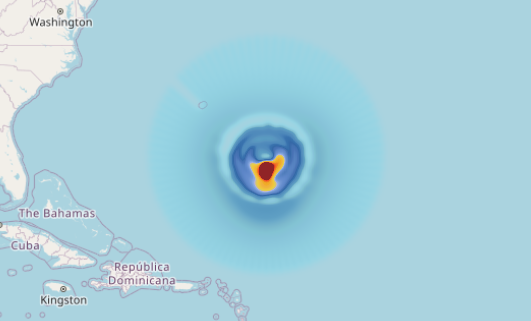
\includegraphics[width=0.75\linewidth]{images/heatmap.png}
    \caption{Visualizzazione dei dati generati su mappa (HeatMap)}
    \label{fig:preview-heatmap}
\end{figure}

Una breve anteprima dei dati testuali generati:

\begin{table}[ht]
\centering
\label{tab:data}
\begin{tabular}{
    S[table-format=2.15]
    S[table-format=-2.1]
    S[table-format=2.15]
    S[table-format=4.0]
    S[table-format=4.15]
    S[table-format=1.1]
}
\toprule
{Latitude} & {Longitude} & {Value} & {Bathy1} & {Bathy2} & {Sector} \\
\midrule
37.25897980148502 & -59.3 & 88.04606789424417 & 1003 & 5163.03076171875  & 0.0 \\
37.24995686563234 & -59.3 & 88.04978137920247 & 2007 & 5167.09033203125  & 0.0 \\
37.24093392977967 & -59.3 & 88.05349035487939 & 3011 & 5166.5244140625   & 0.0 \\
37.231910993927   & -59.3 & 88.05719509329765 & 4015 & 5166.5576171875   & 0.0 \\
37.22288805807432 & -59.3 & 88.06089653237328 & 5019 & 5166.21142578125  & 0.0 \\
37.21386512222165 & -59.3 & 88.06459277272671 & 6022 & 5161.037109375    & 0.0 \\
37.20484218636896 & -59.3 & 88.06828474014407 & 7026 & 5158.3720703125   & 0.0 \\
\bottomrule
\end{tabular}
\end{table}

\subsection{Utilità principale}

I risultati generati dal modello permettono di stimare con precisione le aree di maggiore impatto acustico attorno alla sorgente, evidenziando come il rumore si attenui con la distanza seguendo le leggi della propagazione sott'acqua. \cite{airgun_marine_life} 
Grazie all'inclusione di rotte navali e dettagli morfologici come isole, coste e batimetria, il modello è in grado di identificare sia zone con un livello di rumore più elevato, sia zone \say{d'ombra} dove il suono risulta attenuato rispetto all'ambiente circostante.

\noindent In sintesi, il modello trasforma una simulazione fisica complessa in un output geografico e operativo, utile per la gestione responsabile dell'inquinamento acustico marino.

  \chapter{Introduzione e contesto progettuale}
\label{ch:introduzione}

\section{Obiettivo del progetto}

Il presente elaborato descrive le fasi di progettazione e sviluppo del frontend web di un sistema interattivo per la visualizzazione dei dati prodotti da un modello di simulazione del rumore subacqueo
L'obiettivo specifico di questa tesi era fornire al team di ricerca uno strumento accessibile via web che permettesse di caricare i risultati del modello, costituiti da grandi volumi di dati geospaziali, di rappresentarli in maniera chiara su mappa interattiva e consentire un'esplorazione dinamica dei dati, con filtri e livelli di dettaglio variabile.
Il frontend doveva quindi fungere da veste grafica per i risultati del modello, offrendo un'esperienza utente fluida, veloce e comprensibile anche a non esperti in tecnologie web o GIS.


% ## Perchè flask ##

\section{Motivazioni della Scelta di Flask}
\label{ch:flask}

\subsection{Introduzione al Framework}
\textit{Flask} è un \textit{microframework} web scritto in Python, pensato per lo sviluppo rapido di applicazioni web leggere ma estensibili; si è progressivamente affermato come una delle soluzioni più apprezzate nell'ambito dello sviluppo web con Python.  
La filosofia alla base di Flask è quella della semplicità e della flessibilità: il \textit{framework} fornisce solo gli strumenti essenziali per avviare un'applicazione web, lasciando allo sviluppatore la libertà di scegliere e integrare le funzionalità aggiuntive tramite estensioni. \cite{flask-docs}

\textit{Flask} ha rappresentato una scelta strategica per la realizzazione del sistema di \textit{backend} dell'applicazione. La sua leggerezza, unita alla possibilità di estensione mirata e all'ottima documentazione disponibile, ha consentito di sviluppare un'infrastruttura web coerente con le esigenze del progetto, senza introdurre complessità superflue. In un contesto accademico, dove spesso è necessario prototipare rapidamente soluzioni specifiche, un \textit{framework} come \textit{Flask} si rivela uno strumento estremamente efficace.

\begin{listing}[H]
\caption{Codice che inizializza un'istanza minimale di Flask}
\label{lst:minimal-flask} % Il label va all'interno dell'ambiente listing o subito dopo la caption
\begin{minted}{python}
from flask import Flask
app = Flask(__name__)

@app.route('/')
def hello():
    return 'Hello, World!'

if __name__ == '__main__':
    app.run(debug=True)
\end{minted}
\end{listing}

\subsection{Vantaggi Offerti}
\subsubsection*{Leggerezza e rapidità di sviluppo}
Uno dei principali punti di forza di Flask risiede nella sua struttura minimale, come si può osservare nel frammento di codice presente nel Listing \ref{lst:minimal-flask}. L'avvio di un'applicazione richiede pochissime righe di codice, rendendo il \textit{framework} particolarmente adatto per prototipi, applicazioni di piccole e medie dimensioni, o per progetti che necessitano di una fase di sviluppo iniziale particolarmente snella.  
Nel contesto di questo progetto, tale caratteristica ha permesso di concentrare l'attenzione sulle funzionalità specifiche dell'applicazione, riducendo al minimo la complessità architetturale.

\subsubsection*{Modularità e facilità di integrazione}
Flask si contraddistingue per un sistema modulare che consente di estendere il comportamento dell'applicazione in modo selettivo. \cite{flask-docs}

Questa flessibilità ha rappresentato un vantaggio significativo, poiché ha consentito l'integrazione fluida con il progetto sviluppato dal collaboratore.

\section{Sfide tecniche e problematiche affrontate}

Durante lo sviluppo, è stato evidente come la quantità e complessità dei dati da trattare richiedesse una notevole attenzione sia in fase di progettazione dell'interfaccia, sia nella scelta delle tecnologie di visualizzazione. Le principali sfide sono rappresentate da:

\begin{itemize}
  \item la gestione di \textit{dataset} composti da centinaia di migliaia di punti, ciascuno rappresentante un valore acustico in coordinate geografiche precise;
  \item la necessità di interagire in tempo reale con la mappa (zoom, pan, click, overlay);
  \item la compatibilità con diversi browser, dispositivi e risoluzioni.
\end{itemize}

A queste problematiche si è aggiunta la difficoltà di conciliare un'interfaccia ricca di funzionalità con un impatto visivo semplice e pulito, mantenendo al contempo un'elevata responsività dell'applicazione.

\subsection{Impatto delle dimensioni del DOM sulle performance}

Uno degli aspetti fondamentali da considerare nello sviluppo di interfacce web interattive è la gestione efficiente del \textit{Document Object Model} (DOM). Il DOM rappresenta la struttura gerarchica di un documento HTML o XML, permettendo ai linguaggi di scripting, come JavaScript, di accedere e manipolare dinamicamente il contenuto, la struttura e lo stile della pagina.

Quando un browser carica una pagina web, inizia analizzando il file HTML per costruire il DOM. Un DOM di grandi dimensioni implica che il browser debba elaborare un numero elevato di nodi, aumentando il tempo necessario per il parsing e la costruzione della struttura interna della pagina. Questo processo può rallentare significativamente il tempo di caricamento iniziale della pagina, specialmente su dispositivi con risorse limitate.

Secondo le linee guida fornite da strumenti come Lighthouse, una pagina web dovrebbe evitare di avere un DOM con più di 1.500 nodi, una profondità massima superiore a 32 livelli o più di 60 nodi figli per elemento. Superare queste soglie può indicare una struttura DOM eccessivamente complessa, con potenziali impatti negativi sulle prestazioni e sull'usabilità della pagina. \cite{chrome-dom-size}

\subsection{Limitazioni nella renderizzazione di molti punti in una pagina HTML}

Uno dei problemi principali emersi fin da subito è stato l'elevato numero di marker da visualizzare sulla mappa. Ogni punto prodotto dal modello corrispondeva a una coordinata geografica e a un valore numerico (in questo caso, il livello di pressione acustica). Visualizzare tutti questi punti contemporaneamente in una pagina web porta inevitabilmente a un sovraccarico del DOM.

Infatti, molti motori di \textit{mapping} web (come Leaflet o Folium) aggiungono un elemento HTML per ogni marker. Questo approccio è sostenibile fino a qualche migliaio di elementi; superata una certa soglia, si assiste a rallentamenti importanti, consumo elevato di RAM e CPU e talvolta al blocco del browser. \cite{folium-react}


\section{Ottimizzazioni adottate}

\subsection{Strategie per mitigare gli effetti di un DOM di grandi dimensioni}

Per rendere possibile la visualizzazione fluida di questi dati, sono state prese in considerazione librerie per mappe che adottano diverse strategie di ottimizzazione, in particolare:

\begin{itemize}
  \item \textbf{Clustering dei marker}. L'adozione di tecniche di \textit{clustering} automatico consente di aggregare dinamicamente i \textit{marker} (o \textit{datapoints}) più vicini tra loro e rappresentarli con un'unica icona contenente un contatore. 
  
  Questo riduce drasticamente il numero di elementi DOM attivi, migliorando la performance percepita. Diverse librerie, come \texttt{Leaflet.markercluster}, permettono questo tipo di ottimizzazione in modo trasparente per l'utente \cite{leaflet-clustering}. Questo concetto può essere esteso anche alle librerie che implementano una Heatmap, dove viene gestito il \textit{clustering} dei \textit{datapoints}.

  \item \textbf{Uso di Canvas e WebGL}. Laddove le performance non erano ancora soddisfacenti, si è proceduto con l'adozione di motori di rendering basati su Canvas 2D e WebGL. 
  
  Queste tecnologie non utilizzano elementi DOM per ciascun marker, ma disegnano direttamente sul contesto grafico, permettendo di visualizzare decine di migliaia di punti mantenendo un'interazione fluida. L'utilizzo di WebGL, in particolare, è stato determinante nei casi con oltre 100.000 punti. \cite{deckgl-webgl}
\end{itemize}
  \chapter{Analisi delle librerie per la visualizzazione di mappe web}

\section{Introduzione}
Le mappe web interattive sono diventate strumenti fondamentali per la visualizzazione e l'analisi di dati geospaziali in ambito scientifico, industriale e ambientale. Con la crescente disponibilità di dataset georeferenziati di grandi dimensioni, la necessità di soluzioni web performanti e flessibili per la loro rappresentazione è oggi più sentita che mai. Negli ultimi anni, lo sviluppo di numerose librerie JavaScript ha reso possibile integrare con relativa facilità mappe interattive all'interno di applicazioni web, offrendo funzionalità avanzate sia per la visualizzazione 2D che 3D.

In particolare, il caso d'uso affrontato in questo lavoro, ossia la rappresentazione di oltre 100.000 punti geolocalizzati, ciascuno associato a un valore di intensità del rumore subacqueo, pone una sfida significativa in termini di rendering e interattività. L'obiettivo principale di questo capitolo è analizzare lo stato dell'arte delle principali librerie JavaScript per la visualizzazione di mappe, con un focus su quelle in grado di gestire grandi volumi di dati mantenendo buone performance grazie al supporto a tecnologie come WebGL \cite{mapbox-gl-js}.

Verranno confrontate le soluzioni più diffuse, sia \textit{open-source} che commerciali, valutandone la modularità, la facilità d'integrazione, e la capacità di offrire un'esperienza utente fluida anche in scenari complessi. Il fine ultimo è individuare la libreria più adatta a essere integrata nel sistema M-NAT, garantendo un'interfaccia reattiva, scalabile e in grado di restituire in modo chiaro e immediato l'informazione acustica elaborata dal modello.

\subsection{Cos'è un Heatmap}
Una \emph{heatmap} è una rappresentazione grafica bidimensionale che utilizza una scala cromatica per visualizzare l'intensità o la concentrazione di un fenomeno all'interno di una griglia o mappa. Le tonalità più calde (es. rosso, arancione) indicano valori più elevati, mentre quelle fredde (es. blu, verde) rappresentano valori più bassi.

Questo tipo di visualizzazione facilita l'individuazione immediata di pattern, cluster o anomalie in insiemi di dati complessi, risultando particolarmente utile in ambiti come l'analisi geospaziale, il web analytics, l'urbanistica, l'economia e la ricerca scientifica. In applicazioni geospaziali, una \emph{spatial heatmap} sovrappone dati di densità geolocalizzata su una mappa, evidenziando visivamente le aree di maggiore concentrazione del fenomeno studiato \cite{vwo-heatmap,heatmap-wikipedia,clarity-heatmap}.


\section{Criteri di valutazione}
Per confrontare le diverse librerie sono stati definiti alcuni criteri fondamentali:
\begin{itemize}
  \item \textbf{Facilità d'integrazione e documentazione}
  \item \textbf{Performance e fluidità dell'interazione}
  \item \textbf{Supporto a dati vettoriali e raster}
  \item \textbf{Licenza e costi d'uso}
  \item \textbf{Compatibilità con altri strumenti e framework}
\end{itemize}

% import leaflet.tex
\section{Leaflet}
\label{ch:leaflet}

\subsection{Facilità d'integrazione e documentazione}  
Leaflet fornisce una guida introduttiva, esempi interattivi e un'API reference completa sul sito ufficiale \cite{leaflet-doc}.  
La curva di apprendimento è bassa grazie a metodi semplici come \texttt{L.map()}, \texttt{L.tileLayer()} e \texttt{L.marker()}, e la comunità mantiene un ampio catalogo di plugin per estendere ogni funzionalità, dal \textit{clustering} dei marker all'integrazione con dataset GeoJSON complessi \cite{react-leaflet}.

\subsection{Performance e fluidità dell'interazione}  
Di default Leaflet usa SVG e elementi DOM per il rendering, garantendo ottime performance fino a 5.000–10.000 feature\cite{supercluster}.  
Per dataset più voluminosi, plugin come \texttt{Supercluster} permettono di raggruppare i punti via \textit{clustering} su struttura R‑tree e riducono drasticamente i marker renderizzati\cite{supercluster}.  
In alternativa, estensioni WebGL come \texttt{leafgl} sfruttano la GPU per mantenere un'interattività fluida anche con decine di migliaia di feature\cite{leafgl}.  

WebGL (Web Graphics Library) è un'API JavaScript per il rendering di grafica 2D e 3D interattiva ad alte prestazioni direttamente nel browser, sfruttando l'accelerazione hardware della GPU \cite{wiki-webgl}.  
Avere supporto a WebGL all'interno di una libreria per mappe web è fondamentale per gestire grandi quantità di dati geospaziali e garantire un'esperienza utente fluida, poiché il carico grafico viene trasferito dalla CPU alla GPU tramite \textit{shader} e buffer dedicati \cite{khronos-webgl}.  
Senza WebGL, il rendering di dataset massivi ricadrebbe sul DOM e sulla CPU, con evidenti rallentamenti e limiti di scala.


\subsection{Supporto a dati vettoriali e raster}  

I \textit{raster} sono un modello di dati spaziali in cui lo spazio geografico viene suddiviso in una griglia regolare di celle (o pixel), organizzate in righe e colonne, e ciascuna cella contiene un valore numerico che rappresenta un fenomeno reale, come temperatura o elevazione. Questi dati derivano spesso da immagini digitali, fotografie aeree, satellitari o mappe scannerizzate, e sono particolarmente adatti a rappresentare variabili continue distribuite su un'area. \cite{esri-raster-model,qgis-raster-data}

La gestione dei \emph{raster tiles} (p.es. OpenStreetMap o MapTiler) è immediata con \texttt{L.tileLayer()}\cite{maptiler-raster}.  
Il supporto ai \emph{vector tiles} non è nativo, ma può essere aggiunto tramite plugin consolidati come \texttt{leaflet-geojson-vt} e \texttt{Leaflet.VectorGrid}, che frammentano i grandi file GeoJSON/TopoJSON in tile \textit{client‑side} per un caricamento e un clipping più efficienti \cite{leaflet-geojson-vt,vectorgrid}.  

\subsection{Licenza e costi d'uso}  
Leaflet è rilasciato sotto licenza BSD2‑Clause (Simplified) e BSD3‑Clause, entrambe estremamente permissive e compatibili con progetti commerciali senza obblighi di royalty.
Non esistono canoni d'uso; per chi desidera supporto professionale, sono disponibili piani di consulenza e SLA a pagamento offerti da terze parti. \cite{leaflet-doc, leaflet-license}

\subsection{Compatibilità con altri strumenti e framework}  
Viene concepita inizialmente come libreria JavaScript; per React esiste \texttt{ReactLeaflet}, una raccolta di componenti che incapsulano mappe Leaflet in JSX e ne semplificano l'uso all'interno di applicazioni React. \cite{react-leaflet}

\newpage
\section{Mapbox GL}
\label{ch:mapbox}

\subsection{Facilità d'integrazione e documentazione}  
Mapbox GL JS è una libreria JavaScript client-side che sfrutta WebGL per costruire mappe interattive direttamente nel browser.  
La documentazione ufficiale è organizzata in guide passo‑passo e in una API reference dettagliata, entrambe mantenute costantemente aggiornate sul sito Mapbox.  
L'installazione può avvenire tramite CDN o, per un'integrazione nei workflow moderni, installando il pacchetto \texttt{mapbox-gl} con npm o yarn. \cite{mapbox-docs}  

\subsection{Performance e fluidità dell'interazione}  
Grazie al rendering GPU‑accelerato, Mapbox GL JS è in grado di mantenere un frame rate elevato anche con centinaia di migliaia di feature.
Le metriche principali per misurare le prestazioni sono il \emph{render time}, il \emph{source update time} e il \emph{layer update time}, tutte analizzabili tramite logging interno.  
Per dataset estremamente grandi è possibile ottimizzare i tileset applicando tecniche di \emph{tile clipping} e caching client-side, come descritto nella guida ufficiale ai \textit{vector tiles} \cite{mapbox-vector, article-highperf}.  

\subsection{Supporto a dati vettoriali e raster}  
Mapbox GL JS supporta nativamente i \emph{vector tiles} in formato MVT, uno standard basato su Google Protobuf per file con estensione \texttt{.mvt}\cite{mapbox-vector}.  
Il caricamento di \emph{raster tiles} da terze parti è altrettanto semplice: basta definire una sorgente di tipo \texttt{raster} e aggiungere il layer corrispondente, seguendo gli esempi forniti nella documentazione \cite{mapbox-raster}.  

\subsection{Licenza e costi d'uso}  
A partire dalla versione 2, Mapbox GL JS è distribuito sotto licenza commerciale e richiede un \textit{token} Mapbox per l'uso in produzione.  
Il modello di pricing è basato sui \emph{map loads} mensili, con una soglia gratuita di base e piani a consumo che scalano automaticamente con l'utilizzo \cite{mapbox-license-v2, mapbox-pricing}.  

\subsection{Compatibilità con altri strumenti e framework}  
In ambito React è disponibile \texttt{react-map-gl}, una raccolta di componenti che semplifica l'integrazione di Mapbox GL JS in applicazioni basate su React \cite{react-map-gl,mapbox-react-tutorial}.  

Per analisi spaziali avanzate è possibile combinare Mapbox GL JS con librerie come Turf.js, aggiungendo operazioni geospaziali direttamente sul client.  
Chi volesse implementare visualizzazioni 3D o modelli personalizzati può estendere la mappa con Three.js tramite un CustomLayer.  
Infine, Mapbox offre SDK nativi per iOS e Android, che permettono di riutilizzare stili e tileset MVT nelle applicazioni mobile con API coerenti \cite{mapbox-ios, mapbox-mobile-sdk}.  

\newpage
\section{Deck.gl}
\label{ch:deckgl}

\subsection{Facilità d'integrazione e documentazione}  
Deck.gl è un framework GPU‑powered pensato per la visual exploratory data analysis di grandi dataset geospaziali.  
La documentazione ufficiale, disponibile sul sito di Deck.gl (https://deck.gl/docs), include un'introduzione, guide passo‑passo e una API reference completa, oltre a esempi di codice e uno showcase interattivo \cite{deckgl-docs}.  
L'installazione è semplice: basta aggiungere il pacchetto \texttt{deck.gl} da npm o yarn, oppure includere i bundle via CDN \cite{deckgl-npm,deckgl-github}.  

\subsection{Performance e fluidità dell'interazione}  
Grazie al rendering WebGL2 (e supporto sperimentale a WebGPU), Deck.gl mantiene frame rate elevati anche con milioni di punti: per esempio, lo \texttt{ScatterplotLayer} rimane fluido fino a circa 1M di elementi su hardware consumer, degradando in modo controllato oltre i 10M \cite{deckgl-performance}.  
Demo storiche mostrano la visualizzazione di oltre 2M di punti e 36K viaggi in tempo reale con interpolazione GPU di New York City \cite{deckgl-uber-blog}.  
Il core di Deck.gl è ottimizzato per il caricamento e l'aggiornamento dei dati a livello di tile, riducendo la pressione sulla CPU e sfruttando in modo efficiente la GPU \cite{deckgl-github}.  

\subsection{Supporto a dati vettoriali e raster}  
Deck.gl offre una vasta libreria di layer per dati vettoriali; fra i più rilevanti abbiamo: 

\begin{itemize}
    \item \texttt{GeoJsonLayer},
    \item \texttt{MVTLayer}
    \item \texttt{VectorTileLayer}
\end{itemize}

Queste librerie consentono di caricare GeoJSON e Mapbox Vector Tiles in MVT con clipping e streaming dinamico\cite{deckgl-vector,deckgl-mvtlayer}.  
Per i raster tiles, il plugin \texttt{deck.gl-raster} e il layer \texttt{RasterTileLayer} (in Carto integration) permettono di visualizzare immagini satellitari o DEM con WebGL direttamente nel canvas di Deck.gl.  
L'architettura a layer composabili facilita anche l'estensione a casi d'uso personalizzati, integrando WebGL modules per elaborazioni \textit{on-the-fly} di dati raster avanzati\cite{deckgl-maptiler,deckgl-raster-plugin}.  

\subsection{Licenza e costi d'uso}  
Deck.gl è rilasciato con licenza permissiva MIT, che ne consente l'uso, la modifica e la ridistribuzione anche in progetti commerciali senza royalty. \cite{deckgl-license}  
Non ci sono costi di licenza; l'unico requisito è l'attribuzione del copyright e la preservazione del testo di licenza originale.  

\subsection{Compatibilità con altri strumenti e framework}  
Deck.gl offre una buona integrazione con React tramite il componente \texttt{@deck.gl/react}, che espone \texttt{DeckGL} e hooks per gestire view state e interazioni in JSX. \cite{deckgl-react}  
Per altri framework, la comunità mantiene binding e plugin non ufficiali (ad es. Vue, Angular) raccolti in \texttt{deck.gl-community}, benché con supporto meno costante. \cite{deckgl-community}
Il layer system di Deck.gl è inoltre progettato per lavorare insieme a librerie di analisi spaziale come Turf.js e a motori di rendering 3D come Three.js attraverso CustomLayer. cite{deckgl-faq}

\newpage
\section{OpenLayers}
\label{ch:openlayers}

\subsection{Facilità d'integrazione e documentazione}
OpenLayers mette a disposizione una documentazione ufficiale molto dettagliata, con guide introduttive, esempi interattivi e API reference sul sito del progetto \cite{openlayers-doc}.  
Il codice sorgente e il tracker delle issue sono ospitati su GitHub, dove si trova anche il file di licenza Clear BSD 2‑Clause.
È inoltre attivo un ecosistema di wrapper e plugin non ufficiali raccolti in repository quali \say{awesome-openlayers} \cite{openlayers-github,awesome-openlayers}.

\subsection{Performance e fluidità dell'interazione}
Il supporto WebGL in OpenLayers permette di sfruttare la GPU per il rendering di geometrie complesse: esempi ufficiali mostrano come il layer \texttt{WebGLVectorLayer} mantenga un frame rate elevato anche con decine di migliaia di punti. \cite{openlayers-webgl-example} 
Workshop dedicati illustrano tecniche di ottimizzazione, come il tiling client‑side e la gestione dinamica dei dati, per mantenere interactive performance anche in scenari di grandi dataset.
Discutere problemi di performance su forum come GIS StackExchange rivela strategie quali clustering e buffer dinamici per ridurre il carico di rendering. \cite{openlayers-webgl-workshop,openlayers-issue-perf}

\subsection{Supporto a dati vettoriali e raster}
\subsubsection*{Vector tiles}
OpenLayers supporta nativamente Mapbox Vector Tiles (MVT) tramite il layer \texttt{VectorTileLayer}, consentendo styling lato client e caricamento tile‑by‑tile.
Sono disponibili esempi per OSM Vector Tiles che utilizzano il formato MVT per ottenere ottime prestazioni con dataset di medie dimensioni. \cite{openlayers-mapbox-vector-tiles,openlayers-osm-vector-tiles}

\subsubsection*{Raster tiles}
Il framework gestisce tile raster da sorgenti XYZ e WMS con le classi 

\begin{itemize}
    \item \texttt{ol/source/XYZ} 
    \item \texttt{ol/source/TileWMS}
\end{itemize}

semplificando l'uso di basemap come OpenStreetMap o servizi Geoserver\cite{openlayers-raster-xyz}.  
Per casi avanzati, la documentazione ufficiale risulta un'importante risorsa per ottenere più informazioni sulla riproiezione dei raster.

\subsection{Supporto a WebGL}
Il motore WebGL di OpenLayers, accessibile tramite \texttt{WebGLPointsLayer} e \texttt{WebGLVectorLayer}, sfrutta buffer di vertici e shader GLSL per trasferire gran parte del lavoro di rendering alla GPU, rendendo possibile la visualizzazione di grandi moli di dati con animazioni fluide. \cite{openlayers-webgl-example,openlayers-webgl-workshop}

\subsection{Licenza e costi d'uso}
OpenLayers è rilasciato sotto licenza Clear BSD 2‑Clause, una licenza permissiva che permette uso, modifica e ridistribuzione anche in progetti commerciali senza royalty \cite{openlayers-github,ol-cesium-license}.  
Non sono previsti costi di licenza, ma il progetto invita a donare tramite OSGeo per sostenere il mantenimento del software \cite{openlayers-doc}.

\subsection{Compatibilità con altri strumenti e framework}
Oltre a React, la comunità ha sviluppato binding per Vue, Angular e GWT, elencati nella pagina \say{Useful 3rd party libraries} del sito ufficiale.  
Per analisi spaziale lato client è comune integrare OpenLayers con Turf.js, come mostrato nell'esempio ufficiale \say{\texttt{turf.js}} \cite{awesome-openlayers,openlayers-turf-example}.  

\newpage
\section{Folium}
\label{ch:folium}

\subsection{Facilità d'integrazione e documentazione}  
Folium è una libreria Python che semplifica la creazione di mappe interattive basate su Leaflet direttamente da notebook e applicazioni web \cite{folium-doc}.
La documentazione ufficiale comprende un User Guide con esempi passo‑passo e un'\textit{API Reference} dettagliata, entrambi disponibili sul sito del progetto \cite{folium-userguide}.  
Il \textit{repository} GitHub ospita codice, issue e un elenco di plugin e pacchetti correlati (\textit{xyzservices}, streamlit‑folium) che estendono le funzionalità di base \cite{folium-github,folium-pypistats}.  
Online è facile reperire delle guide pratiche per integrare Folium in workflow di \textit{data science} basati, per esempio, su Jupyter Notebook \cite{folium-tutorial,folium-realpython}.

\subsection{Performance e fluidità dell'interazione}  
Di default Folium rende le feature come oggetti JavaScript nel DOM di Leaflet: ciò è efficiente per qualche migliaio di marker, ma può diventare lento con dataset superiori a 10.000 punti, come evidenziato da una discussione su StackOverflow riguardo al MarkerCluster, dove, per dataset molto voluminosi, viene consigliato di preprocessare i dati in vector tiles o di applicare tecniche di clustering lato server \cite{folium-cluster-issue}.  

Sono disponibili diversi plugin come \textit{MarkerCluster} e \textit{FastMarkerCluster}, mirati a migliorare l'esperienza utente con il crescere della dimensione del dataset \cite{folium-cluster-issue,folium-pypistats}.  
Il numero di download settimanali (più di 500.000) testimonia la diffusione di Folium e la necessità di \textit{best practice} per gestire prestazioni e scalabilità.

\subsection{Supporto a dati vettoriali e raster}  
Folium supporta nativamente diversi tipi di layer vettoriali (GeoJSON, Choropleth, HeatMap) e mette a disposizione \textit{convenience class} per aggiungere popup e tooltip dinamici.  
Il supporto a raster avviene tramite classi come \texttt{TileLayer}, \texttt{WmsTileLayer} e \texttt{ImageOverlay}, permettendo di utilizzare \textit{basemap} OpenStreetMap, mappe satellitari e overlay di immagini o video georeferenziati.  
Per esigenze avanzate di overlay raster in Jupyter, utilizzando \textit{Rasterio} è possibile integrare singole bande \textit{tiff} in mappe interattive. \cite{folium-raster,folium-tutorial, folium-doc}

\subsection{Licenza e costi d'uso}  
Folium è rilasciato sotto licenza MIT, liberamente utilizzabile, modificabile e ridistribuibile anche in contesti commerciali senza alcun costo di licenza.  
La gestione delle dipendenze e dei plugin avviene via PyPI, con aggiornamenti regolari e un ciclo di rilascio che segue le versioni di Leaflet sottostanti \cite{folium-lic,folium-pypi}.

\subsection{Compatibilità con altri strumenti e framework}  
Folium si integra con Jupyter Notebook e JupyterLab, generando mappe HTML \say{\textit{embeddate}} direttamente nelle celle del notebook.  
Esistono \textit{binding} pacchetti per far girare mappe Folium in applicazioni Streamlit (\texttt{streamlit-folium}) e wrapper per framework frontend come React, sebbene in questi casi si usino spesso \textit{iframe} o comunicazione via REST \cite{folium-github,folium-react}.  
L'ecosistema di plugin ospita esempi per l'uso con GeoPandas, Pandas e altri pacchetti di data science, facilitando l'integrazione in pipeline di elaborazione geospaziale \cite{folium-doc,folium-userguide}.

\newpage
\section{\textit{Benchmarking} Automatizzato per il Confronto Prestazionale tra Librerie}

Al fine di condurre un'analisi comparativa rigorosa e sistematica delle prestazioni offerte dalle diverse librerie di visualizzazione cartografica prese in esame, è stato realizzato un progetto separato il quale implementa una specifica funzionalità di benchmarking automatizzato. Questo sistema è stato impiegato per acquisire misurazioni quantitative e ripetibili dei tempi di esecuzione e rendering, minimizzando al contempo l'intervento manuale e le potenziali distorsioni da esso derivanti. Si è posta particolare enfasi nel garantire che ogni singola prova venisse eseguita in condizioni operative il più possibile isolate e \say{pulite}, ovvero esenti da interferenze dovute a stati precedenti dell'applicazione o a risorse memorizzate nella cache.
Grazie a tali dati, è stato possibile valutare la reattività di ogni libreria considerata e presentare, in questo elaborato, un'analisi concisa e fruibile.

Il fulcro di questa architettura di test è rappresentato da un'istanza di Flask che mette a disposizione una pagina web dedicata, accessibile tramite l'endpoint applicativo \texttt{/benchmark}. 
È doveroso specificare come in queste misurazioni non è stato incluso \textit{Folium}; tale libreria si differenzia dalle altre per via del suo diverso funzionamento, infatti non è possibile effettuare un \textit{benchmark} significativo tra librerie \textit{server-side rendered} (SSR) e \textit{client-side rendered} (CSR) a causa delle differenze fondamentali nei loro modelli di \textit{rendering} e nei flussi di esecuzione. 

Nello specifico:
\begin{itemize}
      \item Server-Side Rendering (SSR): Il contenuto HTML completo viene generato sul server e inviato al client. Questo approccio consente una visualizzazione immediata del contenuto e una migliore indicizzazione da parte dei motori di ricerca.\cite{peerdh-ssr-csr-comparison}

    \item Client-Side Rendering (CSR): Il server invia una struttura HTML minima, e il browser del client utilizza JavaScript per costruire dinamicamente l'interfaccia utente. Questo può comportare un ritardo nella visualizzazione iniziale del contenuto e richiede che il browser esegua ulteriori elaborazioni.\cite{devto-csr-vs-ssr}
\end{itemize}
  

Il processo di benchmarking si articola nelle seguenti fasi operative fondamentali:

\begin{itemize}[leftmargin=*]
    \item \textbf{Caricamento Iterativo e Contestualizzato delle Mappe:}
    Per ogni libreria inclusa nel ciclo di test e per ciascuna iterazione configurata, la corrispondente pagina web dedicata alla visualizzazione della mappa (ad esempio, \texttt{/leaflet}, \texttt{/openlayers}, ecc.) viene caricata dinamicamente all'interno di un elemento HTML \texttt{<iframe>}. Quest'ultimo è integrato nella pagina di \textit{benchmark} e serve a creare un ambiente di esecuzione \textit{sandboxed} per ogni test. Questo approccio consente di caricare, inizializzare e renderizzare ogni mappa in un contesto di DOM e JavaScript relativamente isolato, riducendo le possibili interferenze tra test successivi. Sebbene l'\textit{iframe} possa essere configurato per essere invisibile durante l'esecuzione standard, la sua visibilità può essere attivata a fini diagnostici e di \textit{debug}.

    \item \textbf{Implementazione di Strategie Anti-Cache Robuste:}
    Una criticità fondamentale nei test di performance web è l'influenza della cache del browser. Per assicurare che ogni caricamento della mappa avvenga ex novo, attingendo le risorse direttamente dal server (o dalla rete, nel caso di \textit{CDN} esterne), sono state implementate due strategie anti-\textit{cache} complementari e sinergiche:
    \begin{itemize}
        \item \textit{Direttive HTTP Server-Side:} Il server applicativo Flask è stato configurato per apporre, a tutte le risposte HTTP generate, specifiche intestazioni di controllo della cache. Tra queste, le più interessanti sono \texttt{Cache-Control: no-cache, no-store, must-revalidate}, \texttt{Pragma: no-cache}, e \texttt{Expires: 0}, le quali istruiscono esplicitamente il browser a non riutilizzare versioni precedentemente memorizzate delle risorse, ma a richiederle nuovamente.
        \item \textit{Parametrizzazione Dinamica degli URL Client-Side:} In aggiunta alle direttive server-side, un meccanismo di \say{\textit{cache busting}} è applicato lato client. Ad ogni URL della pagina mappa da caricare nell'\textit{iframe} viene programmaticamente aggiunto un parametro di query univoco, tipicamente basato sul \textit{timestamp} corrente (es. \texttt{?t=xxxxxxxxxxxxx}). Questa tecnica rende ogni richiesta URL formalmente distinta dalla precedente agli occhi del browser, contribuendo significativamente a vanificare i meccanismi di \textit{caching} più aggressivi.
    \end{itemize}

    \item \textbf{Raccolta Differita e Asincrona delle Metriche di Performance:}
    La misurazione effettiva delle prestazioni è delegata a ciascuna singola pagina di visualizzazione della mappa. All'interno dello script di ogni pagina mappa (es. \texttt{leaflet.html}), vengono utilizzati meccanismi di timing ad alta precisione, come \texttt{performance.now()}, per registrare gli istanti di inizio e fine delle operazioni chiave: recupero dei dati, inizializzazione della mappa base e rendering dello strato \textit{heatmap}.
    Una volta che tutte queste operazioni sono concluse e le metriche sono state calcolate, la pagina mappa ospitata nell'\textit{iframe} emette un evento JavaScript personalizzato, denominato \texttt{benchmarkMetricsReady}, sull'oggetto \texttt{window} del proprio contesto. Il \textit{payload} associato a questo evento (\texttt{event.detail}) è un oggetto JSON contenente tutte le metriche rilevate (per esempio \texttt{dataFetchTime\_ms}, \texttt{mapInitAndHeatmapRenderTime\_ms}, \texttt{totalClientLoadTime\_ms}, \texttt{totalPoints}). La pagina genitore \texttt{/benchmark} si pone in \textit{ascolto attivo} di questo specifico evento proveniente dall'\textit{iframe}, per poter intercettare e registrare i dati di performance non appena disponibili.

    \item \textbf{Aggregazione, Formattazione e Persistenza dei Dati:}
    Le metriche raccolte per ogni singola iterazione di test vengono progressivamente accumulate in una struttura dati (un array JavaScript) nella pagina \texttt{/benchmark}. Questa struttura include non solo le misurazioni temporali, ma anche metadati contestuali quali il nome della libreria mappa testata, il numero progressivo dell'iterazione e la stringa completa dello User-Agent del browser che ha eseguito il test.
    Al completamento di tutte le iterazioni per tutte le librerie configurate, l'intero \textit{dataset} di risultati viene serializzato in formato JSON e trasmesso, tramite una richiesta HTTP di tipo POST, a un endpoint server-side dedicato: \texttt{/save\_benchmark\_data}. Questo endpoint, gestito dall'applicazione Flask, riceve i dati e provvede ad accodarli in modo persistente a un file testuale formattato come CSV (Comma-Separated Values); è possibile consultare un estratto di poche righe di tale file, disposto in Tabella \ref{tab:csv-metriche-mappe}, in cui viene mostrato come vengono organizzate le misurazioni. Il file, denominato \texttt{benchmarks.csv} e localizzato nella directory radice del progetto, funge da archivio storico di tutte le sessioni di \textit{benchmark}. La sua struttura tabellare, con colonne chiaramente definite, facilita l'analisi successiva e il confronto dei dati, permettendo l'importazione in fogli di calcolo o software statistici.
        
\end{itemize}

\begin{table}[ht]
\centering
\caption{Esempio di dati raccolti per \textit{Leaflet}} % Added descriptive caption
\label{tab:csv-metriche-mappe}
\sisetup{
  output-exponent-marker=\text{\,E\,},
  exponent-product={},
  group-digits=false
}
\begin{tabular}{
  l
  S[table-format=1.0]
  S[table-format=5.0]
  S[table-format=3.2]
  S[table-format=3.0]
}
\toprule
\textbf{Mappa} & \textbf{Iterazioni} & \textbf{Punti totali} & \textbf{Data Fetch (ms)} & \textbf{Map Init \& Render (ms)} \\
\midrule
Leaflet & 1 & 76533 & 502.75 & 580 \\
Leaflet & 2 & 76533 & 487.70 & 561 \\
Leaflet & 3 & 76533 & 480.63 & 546 \\
Leaflet & 4 & 76533 & 468.64 & 536 \\
Leaflet & 5 & 76533 & 462.73 & 539 \\
\vdots  &\vdots  &\vdots  &\vdots  &\vdots \\
Leaflet & 46 & 76533 & 455,67 & 526 \\
Leaflet & 47 & 76533 & 508,65 & 577 \\
Leaflet & 48 & 76533 & 594.60 & 658 \\
Leaflet & 49 & 76533 & 456.62 & 520 \\ 
Leaflet & 50 & 76533 & 499.65 & 568 \\
\bottomrule
\end{tabular}
\end{table}


% focus sul benchmark
\subsection{Metodologia di Rilevamento delle Metriche}

Il sistema di \textit{benchmarking} automatizzato esegue 50 iterazioni per ciascuna libreria cartografica. In ogni iterazione, vengono misurate tre metriche principali: il tempo di recupero dei dati (\textit{data fetch time}), il tempo di inizializzazione e \textit{rendering} della mappa (\textit{map initialization and heatmap render time}) e il tempo totale di caricamento (\textit{total client load time}). Il processo di misurazione inizia quando l'utente richiede la visualizzazione della mappa e termina quando la \textit{heatmap} è completamente renderizzata e interattiva. Per ogni libreria, è stato implementato un sistema di eventi personalizzato che marca con precisione i momenti chiave del ciclo di vita della mappa:

\begin{itemize}
    \item \textbf{Tempo di Recupero Dati}: Misurato dall'inizio della richiesta HTTP fino al completamento del download dei dati dei punti. Questo intervallo è calcolato utilizzando l'API Performance del browser, specificamente attraverso il \texttt{PerformanceNavigationTiming}.

    \item \textbf{Tempo di Inizializzazione e Rendering}: Calcolato dall'istante in cui i dati sono disponibili fino al completamento del rendering della heatmap. Per ogni libreria, questo evento è segnalato in modo specifico:
    \begin{itemize}
        \item \textbf{Leaflet}: Utilizza l'evento \texttt{layeradd} del plugin \texttt{Leaflet.heat} per rilevare l'aggiunta del layer heatmap alla mappa \cite{leaflet-heat}.
        \item \textbf{MapLibre GL JS}: Monitora l'evento \texttt{sourcedata} con controllo dello stato \texttt{loaded} per determinare quando i dati della sorgente sono completamente caricati \cite{maplibre-sourcedata}.
        \item \textbf{OpenLayers}: Sfrutta l'evento \texttt{postrender} del layer heatmap per identificare il completamento del rendering \cite{openlayers-heatmap}.
        \item \textbf{Deck.gl}: Utilizza il callback \texttt{onAfterRender} del componente per rilevare quando il rendering è stato completato \cite{deckgl-onafterrender}.
    \end{itemize}

    \item \textbf{Tempo Totale di Caricamento}: Rappresenta la somma del tempo di recupero dati e del tempo di inizializzazione e rendering, fornendo una metrica complessiva dell'esperienza utente.
\end{itemize}

Riassumendo, ogni iterazione di questo test viene eseguita in un \textit{iframe} isolato per evitare interferenze tra le diverse esecuzioni. Le metriche vengono raccolte lato client attraverso un evento personalizzato \texttt{benchmarkMetricsReady} che viene \textit{dispatchato} al completamento di ogni ciclo di \textit{rendering}. I dati raccolti vengono quindi aggregati e salvati in un file CSV per l'analisi successiva. Questo approccio metodico assicura che le misurazioni siano rappresentative delle reali prestazioni di ciascuna libreria in un contesto applicativo reale.


\subsection{Analisi sulla Correlazione delle Metriche}
\begin{figure}[!ht]
    \centering
    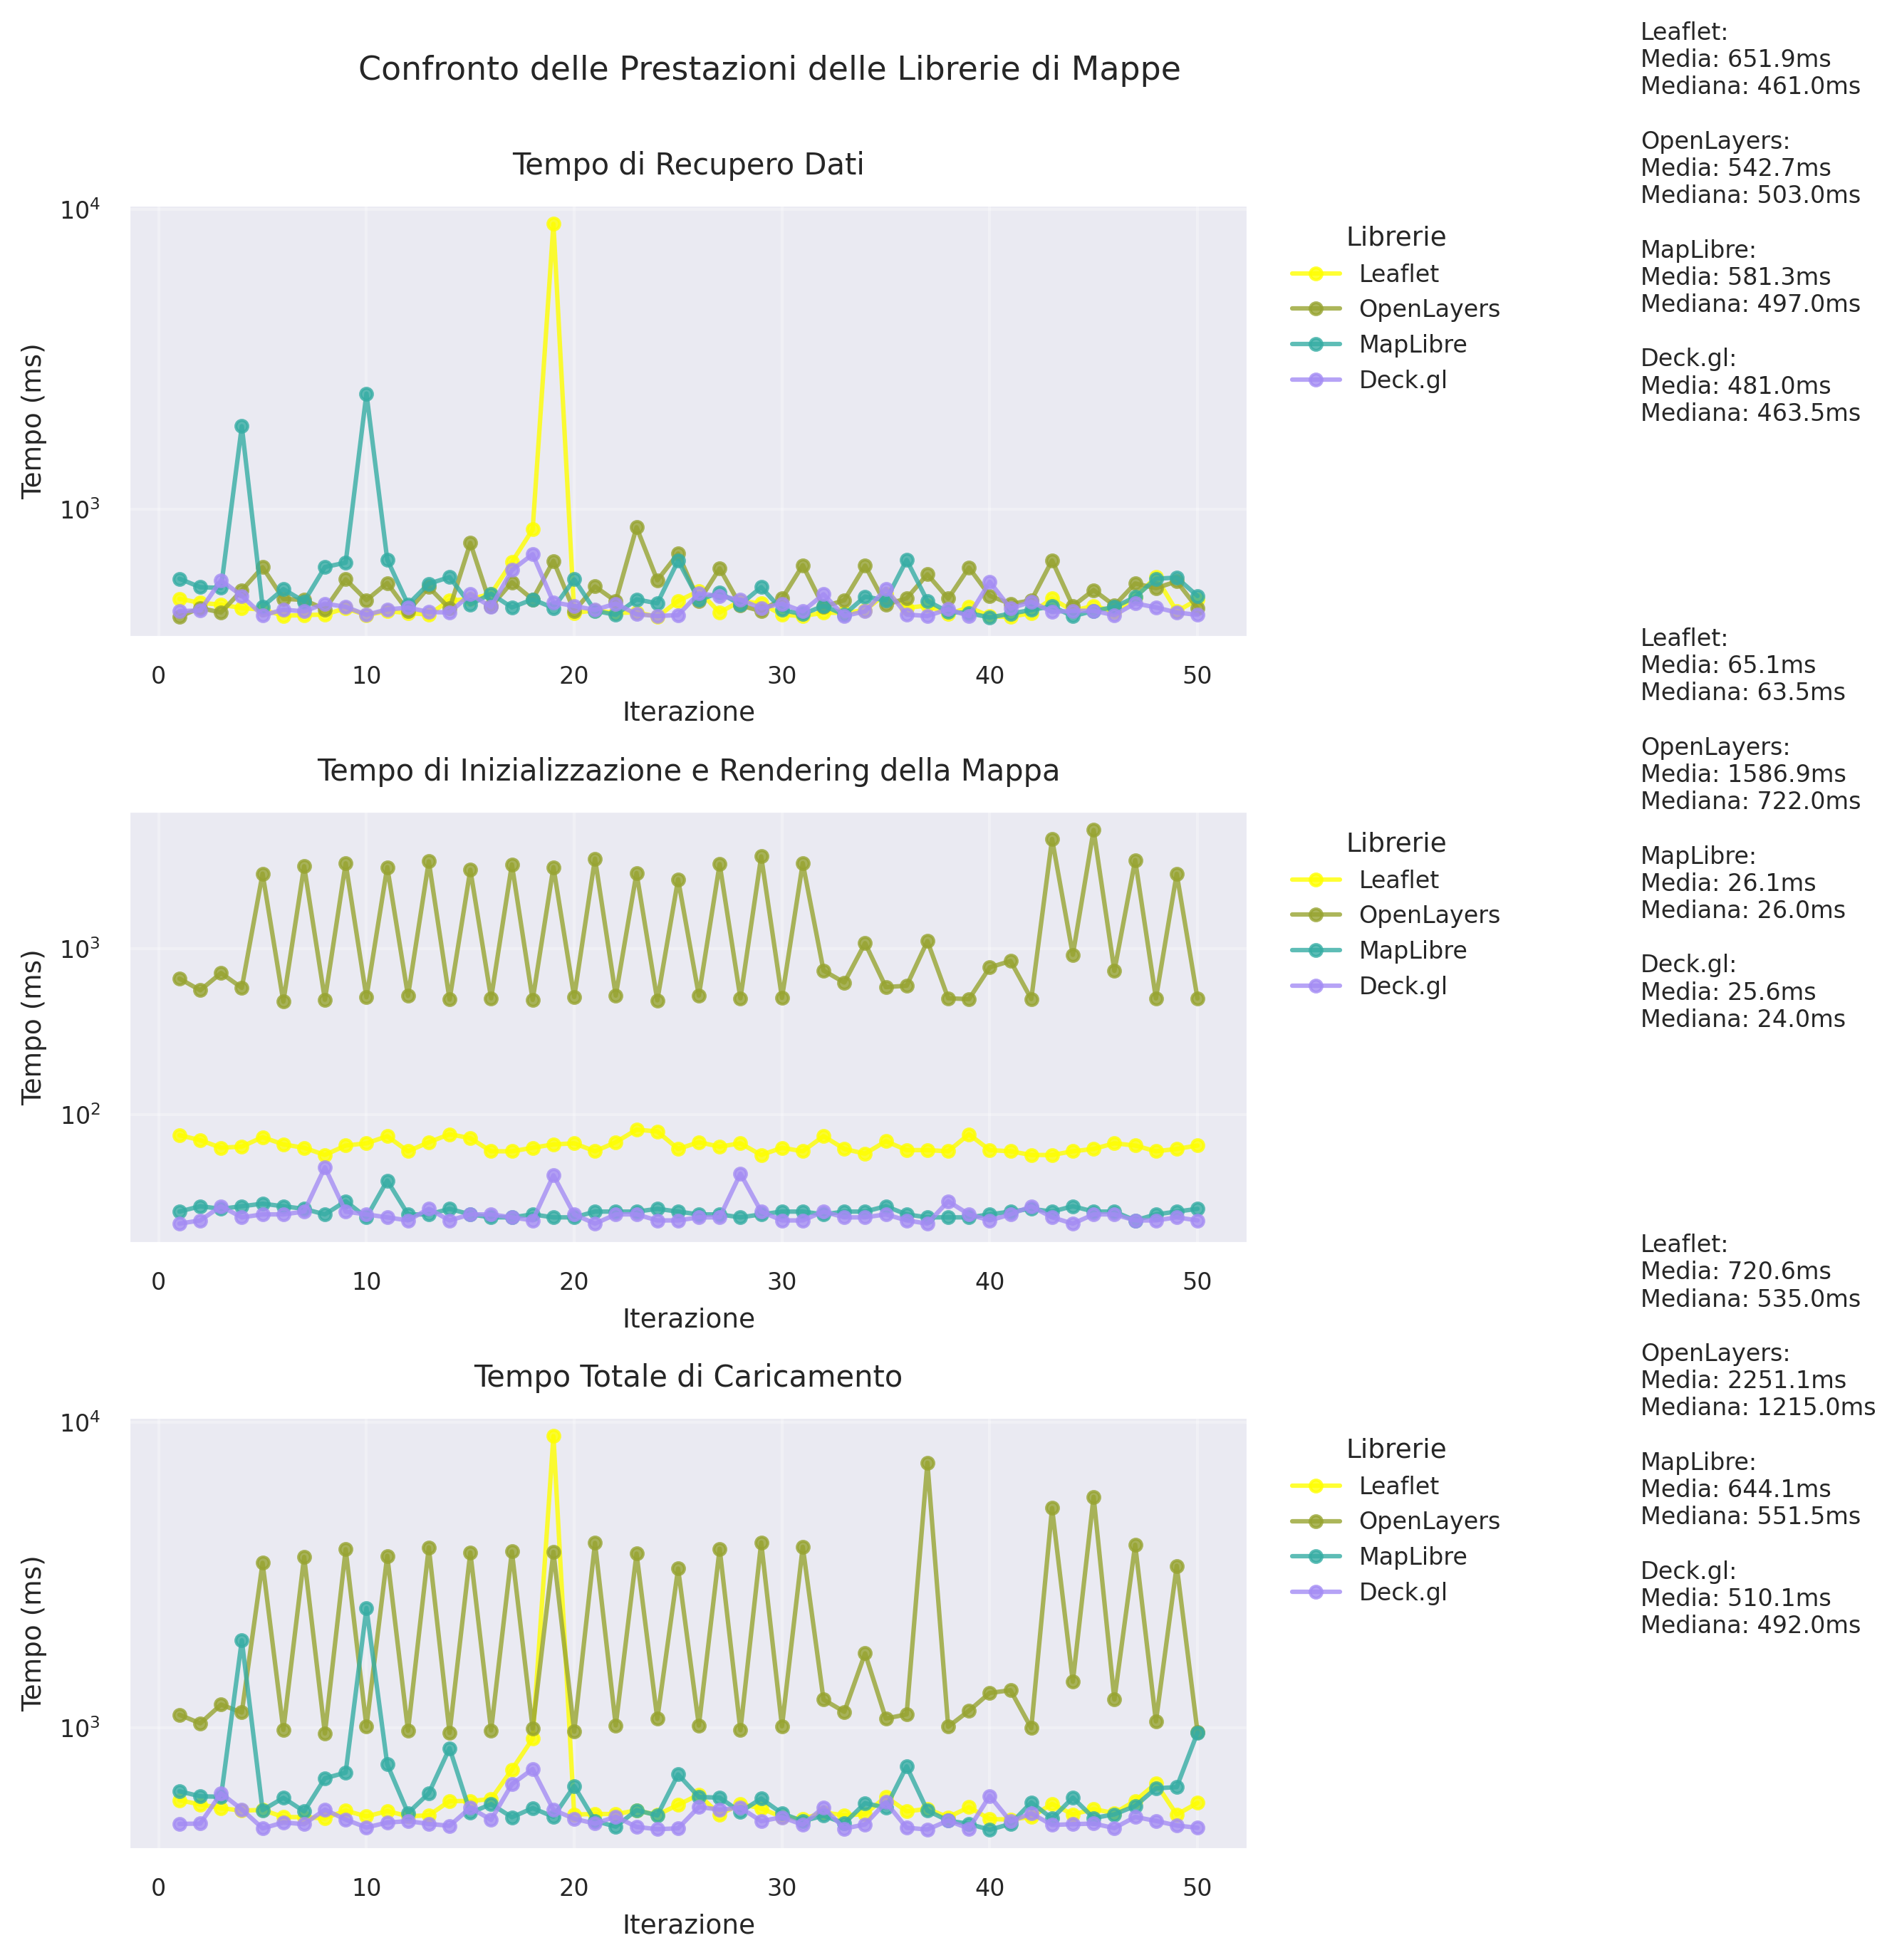
\includegraphics[width=\textwidth]{chapters/librerie-plot/data/confronto_benchmark.png}
    \captionsetup{justification=centering}
    \caption{Grafico combinato di Tempo di caricamento dati,\\ di Inizializzazione Mappa, e Rendering Heatmap}
    \label{fig:map_benchmark}
\end{figure}

\begin{figure}[!ht]
    \centering
    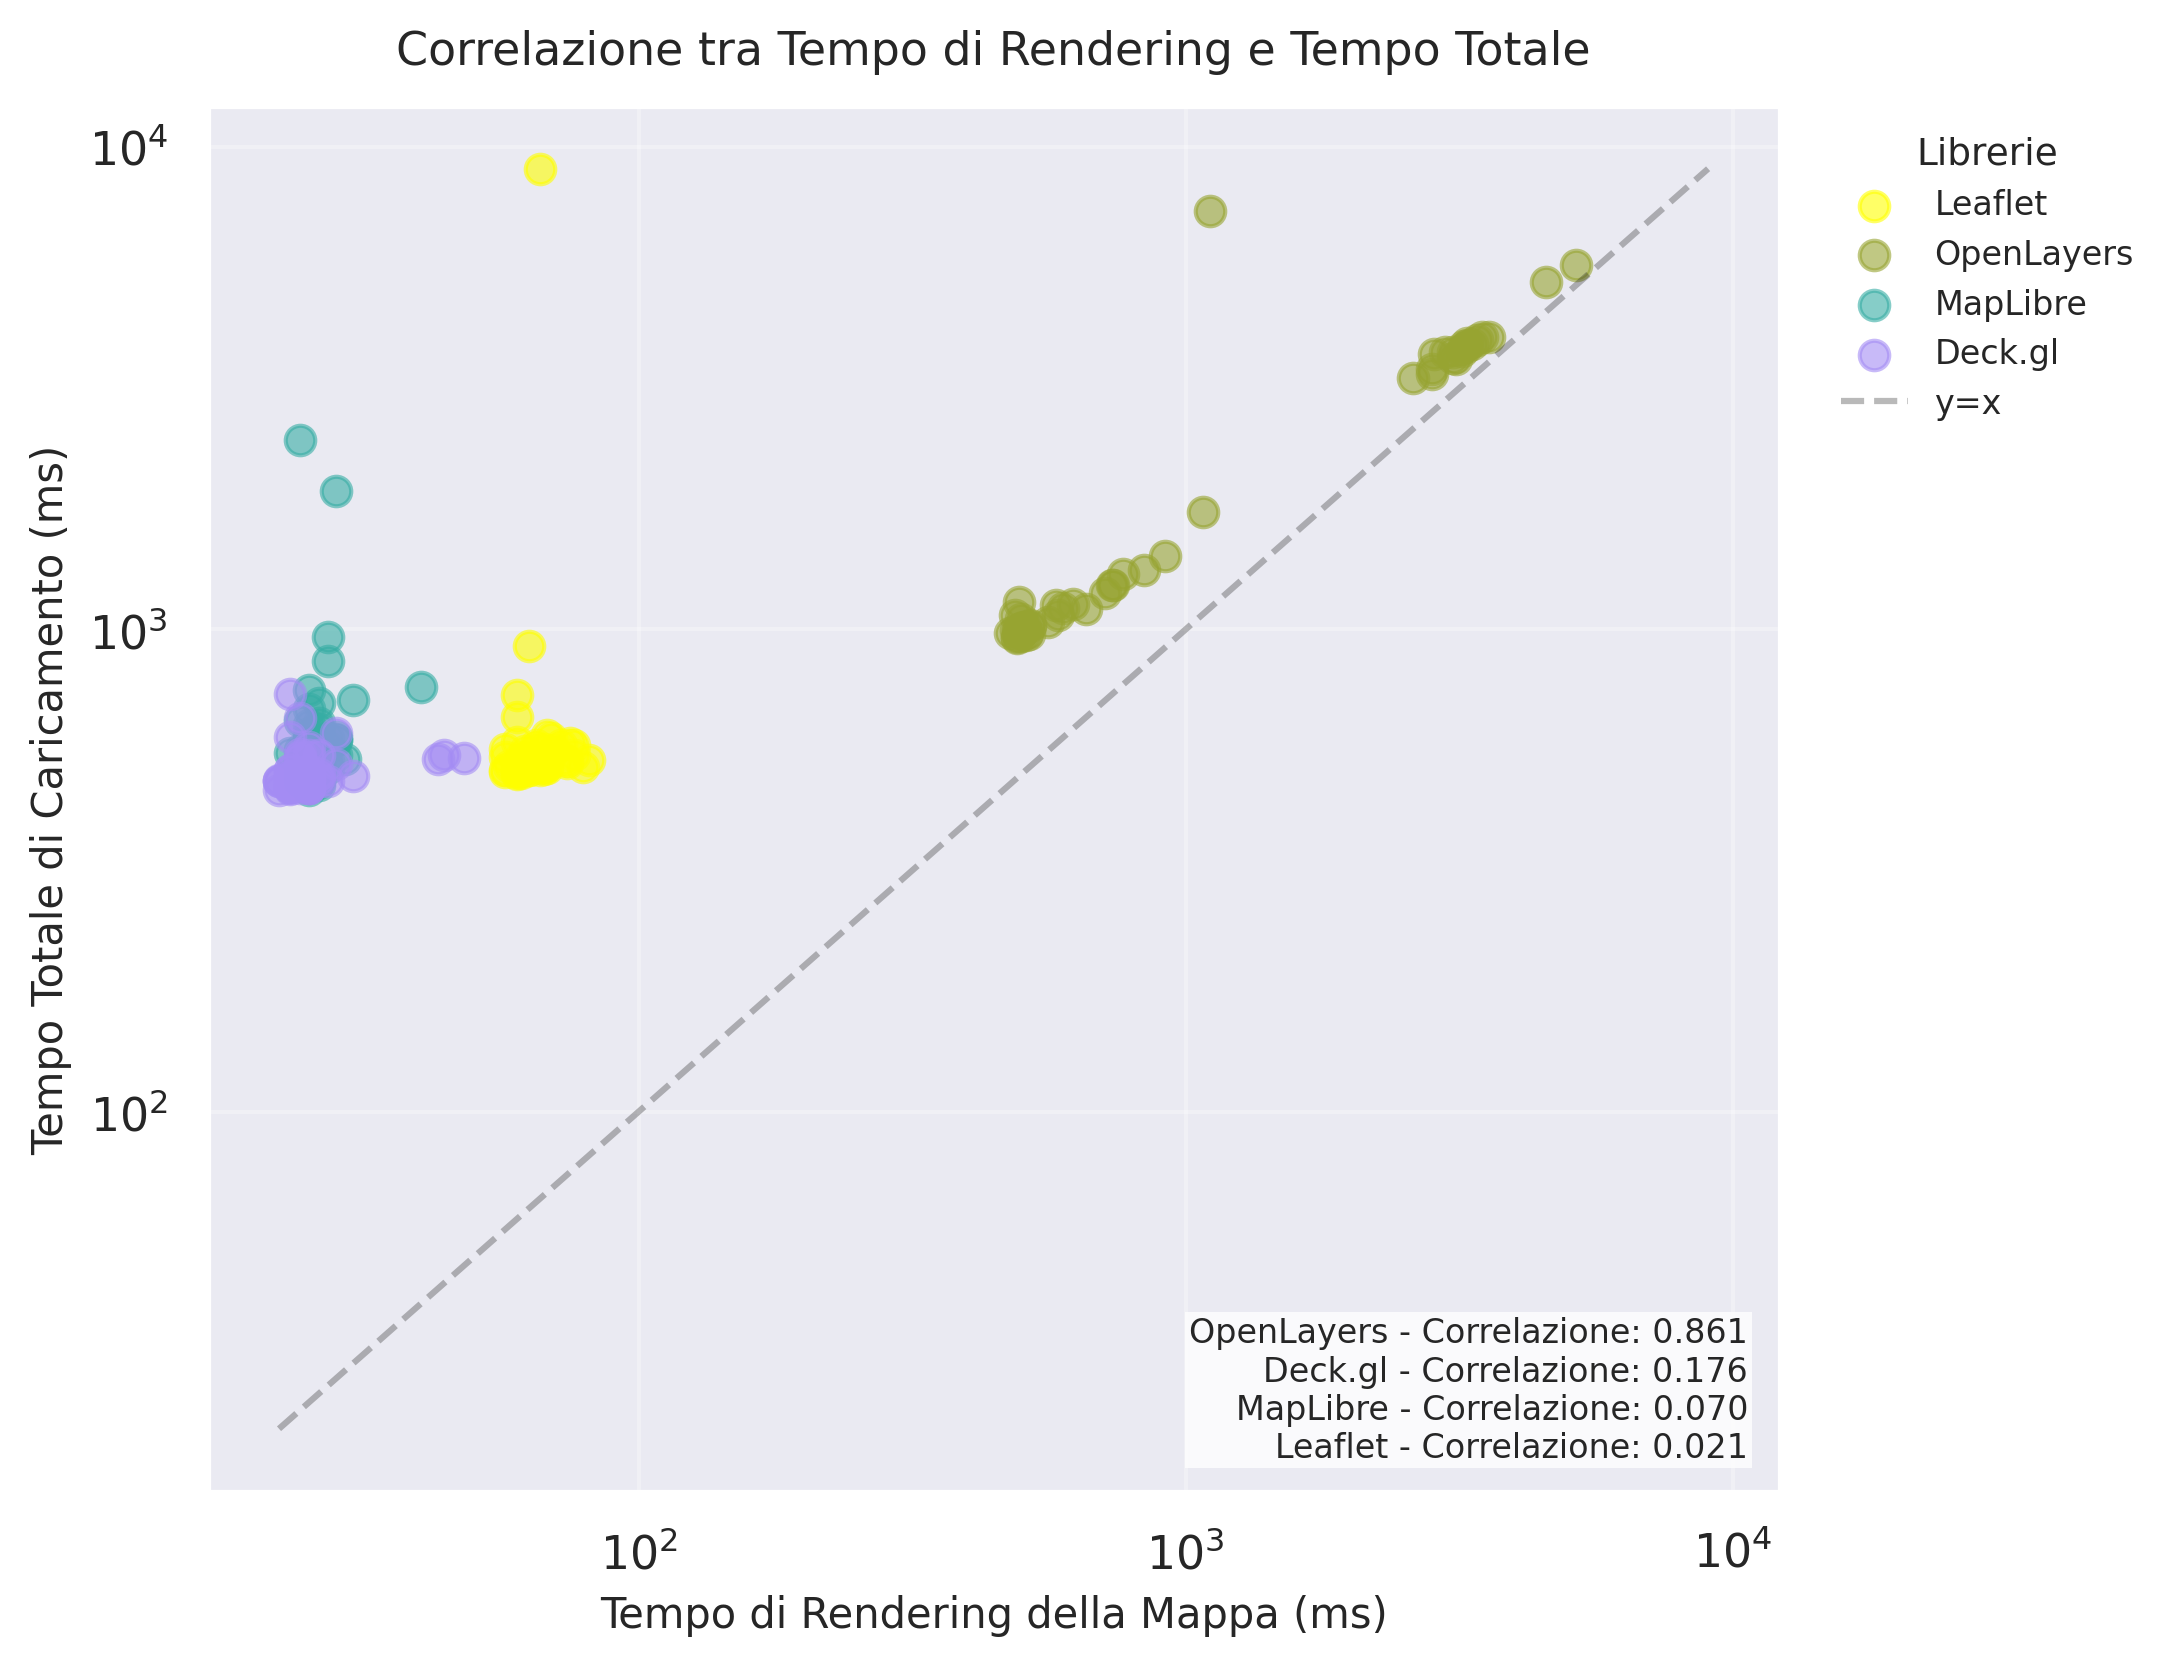
\includegraphics[width=\textwidth]{chapters/librerie-plot/data/correlazione_rendering_totale.png}
    \caption{Grafico che unisce tempo di Inizializzazione Mappa e Rendering Heatmap}
    \label{fig:map_xy_plot}
\end{figure}



% commento grafico linee
Come illustrato in Figura \ref{fig:map_benchmark}, il grafico riassume le prestazioni delle librerie poste in analisi, in relazione alle metriche chiave di caricamento. Le linee presenti nei grafici delineano l'andamento dei dati rilevati e permettono di valutare in modo visivo i punti di forza e di debolezza di ciascuna soluzione.

Nello specifico, il grafico mette a confronto i seguenti dati rilevati:
    \begin{itemize}
        \item Tempo di Recupero dei Dati Geospaziali
        \item Tempo di Inizializzazione e Rendering della Mappa
        \item Tempo totale di Caricamento
    \end{itemize}
    

L'asse \textbf{verticale} rappresenta il tempo in millisecondi impiegato, mentre l'asse \textbf{orizzontale} categorizza la sequenza di rilevazioni ottenute.

Si osserva che le librerie Deck.gl e MapBox/MapLibre eccellono particolarmente nel tempo di inizializzazione e rendering, seguite da Leaflet, registrando i valori più bassi, il che le rende una scelta ottimale per scenari in cui tale aspetto è critico. Al contrario, la libreria OpenLayers mostra prestazioni meno competitive nello stesso ambito, suggerendo aree che richiedono potenziale ottimizzazione o che la rendono meno adatta per carichi di lavoro specifici.

È interessante notare come Leaflet e Deck.gl mostrino prestazioni simili e costantemente basse per il tempo di rendering e OpenLayers presenti una variabilità maggiore per il tempo totale di caricamento. Questo potrebbe indicare fattori architetturali comuni, diverse strategie di ottimizzazione, o impatti di terze parti meno controllabili.

L'analisi di questo grafico di confronto è fondamentale per orientare la scelta della libreria più adatta alle esigenze specifiche del progetto. Essa rivela non solo le performance assolute, ma anche le loro caratteristiche relative, permettendo di identificare la soluzione che meglio si allinea ai requisiti di velocità e reattività dell'applicazione finale.

% commento grafico xy
Ora prendiamo in considerazione ciò che viene illustrato in Figura \ref{fig:map_xy_plot}. Questo  grafico di dispersione presenta la relazione tra il tempo impiegato per il \textbf{rendering della mappa} (misurato in millisecondi sull'asse delle ascisse) e il \textbf{tempo totale di caricamento lato client} (misurato in millisecondi sull'asse delle ordinate). Ogni punto sul grafico rappresenta una singola osservazione di test, e le diverse librerie cartografiche (Leaflet, OpenLayers, MapLibre, Deck.gl), ognuna differenziata da un colore diverso, permettono di distinguere visivamente i loro rispettivi comportamenti.

\begin{itemize}
    \item \textbf{Limite inferiore}
    Si osserva una disposizione dei dati ben definita, dove nessuna libreria è in grado di raggiungere tempi totali di caricamento sotto una certa soglia (indicativamente, $\sim 500$ ms). Interessante la disposizione dei \textit{datapoints} lungo l'asse delle ascisse, quindi l'asse lungo il quale sono disposti i tempi di caricamento in primo luogo della mappa e successivamente del componente \textit{Heatmap}. Ricordo che tale valore è compreso nel più generale tempo di caricamento totale, rappresentato dall'asse delle ordinate; da questo accorgimento si può giustificare l'assenza di \textit{datapoints} situati sotto alla diagonale ipotetica $y=x$.
    
    Le librerie cartografiche che si distinguono per la vicinanza all'origine (Deck.gl, Leaflet, MapLibre) infatti hanno tutte in comune tempi di caricamento dei componenti Mappa e \textit{Heatmap} molto bassi, metrica che può dire la sua nella scelta della libreria per uno specifico caso d'uso.

    \item \textbf{Ulteriori osservazioni}
    Sebbene il grafico in Figura \ref{fig:map_xy_plot} faccia intendere quali siano le librerie generalmente più rapide, è da riconoscere anche un'ulteriore caratteristica: Il grado di correlazione tra i due valori misurati (Tempo di rendering della Mappa e Tempo Totale di Caricamento). Librerie collocate vicino alla diagonale immaginaria $y=x$ sono caratterizzate quindi da una minor differenza tra i due valori misurati. Ciò può indicare un comportamento interessante: in questo caso specifico, abbiamo una libreria (OpenLayers) che impiega più tempo delle altre per il rendering della mappa, ma il tempo di caricamento totale lato \textit{client} risulta poco superiore; questo potrebbe indicare una peggior ottimizzazione lato \textit{Heatmap}, per cui il rendering di tale elemento rappresenta la maggior parte del tempo impiegato dalla libreria per mostrare la mappa a schermo. Un miglioramento su tale versante porterebbe i \textit{datapoints} di tale libreria in una zona più bassa del grafico, probabilmente poco distante dalla diagonale immaginaria. Oppure, adottando una prospettiva più diretta, la libreria nella sua interezza non è tra le più rapide, con o senza \textit{Heatmap}.
    Ed è proprio per via di questa variabilità nell'interpretazione di tale comportamento che i dati riportati in questo grafico risultano utili solamente nell'individuare la libreria generalmente più veloce; è solo dopo aver visivamente accantonato le librerie con tempo totale più elevato delle altre che si è in grado di apprezzare la metrica che valuta il tempo di caricamento della mappa e del componente \textit{Heatmap}.
          
\end{itemize}

In sintesi, l'analisi di questo grafico di correlazione fornisce \textit{insight} preziosi dati sulla dipendenza del tempo di caricamento totale dalle performance di rendering.

\subsection*{Considerazioni sulla Validità e Interpretazione dei Risultati}
È fondamentale sottolineare che, nonostante gli sforzi per standardizzare il processo, le misurazioni di performance nel contesto di un browser web sono intrinsecamente soggette a una certa variabilità. Fattori quali il carico di sistema della macchina ospite, l'attività di altri processi, le specifiche estensioni del browser installate e le fluttuazioni nella latenza di rete (per il recupero di tile e dati) possono influenzare i risultati.
Le specifiche del sistema sul quale sono state effettuate le misurazioni sono brevemente riportate nel frammento di codice nel Listing \ref{lst:inxi_output}.

\begin{listing}[H]
\caption{Output del comando \texttt{inxi}}
\label{lst:inxi_output}
\begin{minted}{bash}
$ inxi
CPU: 8-core AMD Ryzen 7 5800X (-MT MCP-) speed/min/max: 3384/556/4854 MHz
Kernel: 6.15.2-arch1-1 x86_64 Up: 2h 13m Mem: 8.44/15.52 GiB (54.4%)
Storage: 1.6 TiB (30.9% used) Procs: 403 Shell: Bash inxi: 3.3.38
\end{minted}
\end{listing}
  \chapter{Implementazione del progetto}
\label{ch:implementazione}

\section{Introduzione}

Il progetto svolto rappresenta un sistema software avanzato per la visualizzazione e l'analisi di dati geospaziali attraverso mappe di calore interattive. Si tratta di un'applicazione web sviluppata utilizzando tecnologie moderne che combinano potenza computazionale \textit{backend} e interfaccia utente \textit{frontend}.

\section{Analisi dell'Architettura}
\label{ch:backend-architecture}

\subsection{Factory Pattern e Dependency Injection}

Durante lo sviluppo del backend, una delle scelte architetturali fondamentali è stata l'adozione del \emph{Factory Pattern}. Questo pattern è implementato nella funzione \texttt{create\_heatmap\_blueprint()}, che si occupa di generare dinamicamente \textit{blueprint} Flask configurati sulla base di parametri specificati esternamente. L'idea di fondo è che ogni \textit{blueprint} funzioni come un \say{modulo indipendente} che può essere montato o smontato a seconda delle esigenze, mantenendo però coerenza e riusabilità del codice \cite{app-factories}. Il concetto di \textit{blueprint} viene approfondito nella sezione \ref{ss:blueprint}. In altre parole, il backend non è pensato come un'entità rigida, ma come una struttura modulare capace di adattarsi a diversi contesti applicativi semplicemente variando le configurazioni in input. Questo progetto è quindi in grado di inserirsi all'interno di contesti preesistenti e complessi, mediante le giuste accortezze, minimizzando le \say{frizioni} e gli interventi sul codice del progetto che lo ospiterà.

In combinazione con il Factory Pattern, per predisporre il progetto ad essere importato \say{dall'esterno} viene utilizzata anche la tecnica della \emph{dependency injection}, un approccio che permette di fornire componenti esterni (come ad esempio oggetti di configurazione o funzioni di utility) direttamente al momento della creazione del modulo. Questo non solo evita l'uso di variabili globali, spesso fonte di bug e difficoltà nella fase di test, ma rende l'intero sistema più flessibile e facile da mantenere \cite{dependency-injection-wiki,flask-di}.

\subsection{Struttura modulare - Blueprint}
\label{ss:blueprint}

Flask è un \textit{micro‑framework}, tuttavia con la crescita dell'applicazione diventa essenziale una struttura modulare per mantenere il codice chiaro e manutenibile. 
In tale contesto entrano in gioco i \textit{blueprint}, un meccanismo integrato di Flask che consente di suddividere progetti complessi in componenti riutilizzabili e modulari, ognuno dei quali può essere sviluppato, mantenuto e riutilizzato in modo indipendente, permettendo la facile integrazione di futuri \textit{blueprint} senza una riscrittura radicale del progetto principale. 
I \textit{blueprint} permettono di raggruppare rotte, \textit{template} e file statici in \textit{mini}‑applicazioni all'interno della stessa istanza Flask. Essi non sono veri e propri micro‑framework, bensì \textit{insiemi di operazioni} da registrare su un'applicazione principale (anche in più occorrenze). 
Questa metodologia offre diversi vantaggi: \cite{palets_blueprints}

\begin{itemize}
  \item \emph{Modularità e incapsulamento}: ogni \textit{blueprint} contiene logica e risorse legate a una specifica funzionalità (es. visualizzazione mappa, simulazione propagazione, ecc.)
  \item \emph{Scalabilità}: permette di crescere l'app aggiungendo moduli senza impattare il codice esistente.
  \item \emph{Gestione centralizzata}: tutte le configurazioni e le estensioni vengono condivise, mantenendo comunque un ordine strutturale chiaro.
\end{itemize}

\subsubsection{Esempio di Blueprint}

Un \textit{blueprint} è un'entità modulare dichiarata come illustrato nel Listing \ref{lst:flask-blueprint} (es. \texttt{'simple\_page'} importato da \texttt{'templates'}), progettata per incapsulare rotte e risorse di un componente autonomo dell'applicazione.

Dopo la sua definizione, il \textit{blueprint} viene registrato nell'applicazione Flask principale tramite \texttt{app.register\_blueprint()} (Listing \ref{lst:python_blueprint_registration}). Questa operazione lo integra nel contesto runtime dell'applicazione.

Le rotte interne ai \textit{blueprints} sono gestite in modo relativo, prevenendo conflitti di naming con le rotte dell'applicazione principale o di altri \textit{blueprints}. Ciò significa che il percorso completo di una rotta interna dipende dal montaggio del \textit{blueprint}.

\begin{listing}[!ht]
\caption{Codice del file \texttt{simple\_page.py} che descrive un blueprint in Flask}
\label{lst:flask-blueprint} % Il label va all'interno dell'ambiente listing o subito dopo la caption
\begin{minted}{python}
from flask import Blueprint, render_template, abort
from jinja2 import TemplateNotFound

simple_page = Blueprint('simple_page', __name__, template_folder='templates')

@simple_page.route('/<page>')
def show(page):
    try:
        return render_template(f'pages/{page}.html')
    except TemplateNotFound:
        abort(404)
\end{minted}
\end{listing}

Questa gestione relativa permette di \say{montare} il \textit{blueprint} su un percorso \textit{radice} specifico (nell'esempio, su \texttt{/pages} tramite \texttt{url\_PREFIX}), creando un namespace URL logico. Una richiesta a \texttt{<indirizzo principale>/pages} viene quindi internamente instradata al \textit{blueprint}, consentendo un disaccoppiamento che favorisce la modularità e la riusabilità \cite{palets_blueprints}.

\begin{listing}[!ht]
\caption{Blueprint \texttt{simple\_page} montata in /pages}
\label{lst:python_blueprint_registration} % Aggiunto un nuovo label per questo secondo blocco
\begin{minted}{python}
from flask import Flask
from simple_page import simple_page

app = Flask(__name__)
app.register_blueprint(simple_page, url\_PREFIX='/pages')
\end{minted}
\end{listing}

\subsection{Integrazione del blueprint}

Il seguente segmento illustra come, in un progetto terzo basato su Flask, l'integrazione di un sistema di heatmap completo possa essere realizzata con la massima semplicità ed efficienza. L'approccio enfatizza una metodologia \say{zero-configuration} per la configurazione di base, rendendola ideale sia per contesti di prototipazione rapida sia per applicazioni con requisiti standardizzati.
Il cuore di questa integrazione risiede nella funzione \texttt{register\_heatmap()}. Come dimostrato nel codice seguente, l'invocazione di questa funzione con l'istanza dell'applicazione Flask (\texttt{app}) rappresenta l'unico passaggio programmatico richiesto per abilitare l'intera suite di funzionalità di heatmap. Questa astrazione della complessità permetterà agli sviluppatori di concentrarsi sulla logica applicativa principale del loro progetto, delegando la gestione e l'esposizione del modulo heatmap.

\begin{listing}[H]
\caption{Esempio di Integrazione Semplificata della Heatmap in un Progetto Flask}
\label{lst:heatmap_simple_integration}
\begin{minted}{python}
from flask import Flask
from heatmap_blueprint import register_heatmap

app = Flask(__name__)

# Aggiungi qui le tue rotte esistenti
@app.route('/')
def home():
    return "My existing Flask app"

# Aggiungi la funzionalità heatmap
register_heatmap(app)

if __name__ == '__main__':
    app.run(debug=True)
\end{minted}
\end{listing}

A seguito di questa integrazione, supponendo di aver scelto un prefisso per il blueprint (rappresentato dal generico \texttt{URL\_PREFIX}), l'applicazione renderà disponibili automaticamente i seguenti endpoint HTTP, fornendo accesso all'interfaccia utente e ai servizi API della heatmap:

\begin{itemize}
    \item \texttt{http://localhost:5000/} -- Redirect alla dashboard principale.
\end{itemize}

\subsection{Endpoints con Prefisso} % Un sottotitolo per chiarezza
\label{ss:endpoints}

Tutti i seguenti endpoint sono preceduti da \texttt{http://localhost:5000/\{URL\_PREFIX\}/}:

\begin{itemize}
    \item \texttt{} -- Dashboard unificata con heatmap e visualizzazione della propagazione.
    \item \texttt{data} -- Restituisce i dati CSV predefiniti come JSON.
    \item \texttt{data/\{csv\_key\}} -- Restituisce uno specifico dataset come JSON.
    \item \texttt{csv-files} -- Restituisce l'elenco dei file CSV disponibili.
    \item \texttt{config-info} -- Restituisce le informazioni di configurazione e i percorsi auto-rilevati.
    \item \texttt{test-data} -- Testa il caricamento dei CSV e mostra la struttura dei file.
    \item \texttt{static/\{filename\}} -- Serve risorse statiche (auto-rilevate).
\end{itemize}

Questi esempi utilizzano \texttt{http://localhost:5000} per indicare l'indirizzo di accesso locale durante la fase di sviluppo dell'applicazione. L'hostname \texttt{localhost} si riferisce al server in esecuzione sulla macchina locale dello sviluppatore, mentre \texttt{5000} è la porta di default utilizzata dal server di sviluppo integrato di Flask. In un ambiente di produzione, questi URL sarebbero sostituiti dal dominio e dalla porta configurati per il deployment dell'applicazione (es. \texttt{https://mnat.org/heatmap/}).

\newpage


\subsection{Sistema di Configurazione}

Uno dei componenti centrali del sistema è la classe \texttt{HeatmapConfig}, che funge da interfaccia tra l'utente e le configurazioni interne del backend. Questo oggetto è in grado di accettare diverse forme di input: si può passare un singolo file CSV, una lista di file, oppure addirittura un dizionario con nomi personalizzati. Il merito di questa flessibilità è del metodo interno \texttt{\_process\_csv\_files()}, che normalizza i dati contenenti informazioni da disporre sulla mappa in una struttura facilmente gestibile dal resto dell'applicazione.

\begin{listing}[H]
\caption{Costruttore della classe \texttt{HeatmapConfig}}
\label{lst:heatmap_config}
\begin{minted}{python}
class HeatmapConfig:
    def __init__(self, kwargs):
        # Load global configuration defaults first
        global_defaults = self._load_global_defaults()
        
        # CSV file configuration - supports both single file and multiple files
        self.INPUT_CSV_FILE = kwargs.get('INPUT_CSV_FILE', global_defaults.get('INPUT_CSV_FILE', 'data/data.csv'))
        self.CSV_FILES = kwargs.get('CSV_FILES', None)  # New: dict of {name: filepath} or list of filepaths
        self.DEFAULT_CSV = kwargs.get('DEFAULT_CSV', None)  # Which CSV to show by default
        
        # Folder configuration
        self.STATIC_FOLDER = kwargs.get('STATIC_FOLDER', global_defaults.get('STATIC_FOLDER', 'static'))
        self.TEMPLATE_FOLDER = kwargs.get('TEMPLATE_FOLDER', global_defaults.get('TEMPLATE_FOLDER', 'templates'))
        self.COLORS_DIR = kwargs.get('COLORS_DIR', 'colors')
        
        # Data configuration
        self.REQUIRED_COLUMNS = kwargs.get('REQUIRED_COLUMNS', global_defaults.get('REQUIRED_COLUMNS', ['Latitude', 'Longitude', 'Value']))
        self.DEFAULT_MAP_OPACITY = kwargs.get('DEFAULT_MAP_OPACITY', global_defaults.get('DEFAULT_MAP_OPACITY', 0.75))
        self.INITIAL_HEATMAP_RADIUS = kwargs.get('INITIAL_HEATMAP_RADIUS', global_defaults.get('INITIAL_HEATMAP_RADIUS', 40))
        self.INITIAL_HEATMAP_INTENSITY = kwargs.get('INITIAL_HEATMAP_INTENSITY', global_defaults.get('INITIAL_HEATMAP_INTENSITY', 1.5))
        self.INITIAL_HEATMAP_THRESHOLD = kwargs.get('INITIAL_HEATMAP_THRESHOLD', global_defaults.get('INITIAL_HEATMAP_THRESHOLD', 0.00))
        
        # Blueprint configuration (these are blueprint-specific, no global defaults)
        self.URL_PREFIX = kwargs.get('URL_PREFIX', '/heatmap')
        self.BLUEPRINT_NAME = kwargs.get('BLUEPRINT_NAME', 'heatmap')
        
        # Process CSV files configuration
        self._process_csv_files()
\end{minted}
\end{listing}

È possibile scegliere come inizializzare la mappa: se con parametri di default, tramite file di configurazione o tramite parametri passati a \textit{runtime}. La priorità di ogni metodo è differente; abbiamo in ordine decrescente di priorità:

\begin{enumerate}
    \item Parametri passati a \texttt{register\_heatmap()}
    \item File di configurazione config.json globale
    \item Valori di default generici (failsafe)
\end{enumerate}
Nella pratica, questo significa che il sistema può essere utilizzato ed eseguito affidandosi a parametri di default senza una conoscenza profonda del progetto, sia tramite una configurazione granulare dei parametri iniziali. Personalmente, ho trovato molto comodo poter passare da una modalità all'altra senza dover cambiare il codice, ma solo intervenendo sul file \texttt{config.json}.

\begin{listing}[H]
\caption{Metodi per inizializzare la mappa}
\label{lst:register_hm}
\begin{minted}{python}
# Istanza che usa config.json come base
register_heatmap(app, url_prefix='/global')

# Istanza che override specifici parametri
register_heatmap(
    app, 
    CSV_FILES={'Custom': 'data/custom.csv'},
    INITIAL_HEATMAP_RADIUS=60,      # ← Override global default
    url_prefix='/custom'
)
\end{minted}
\end{listing}

L'adozione di questa configurazione gerarchica comporta diversi benefici \cite{dependency-injection-wiki}:

\begin{itemize}
  \item \textbf{Modularità}: le dipendenze sono isolate dal codice, facilitando la sostituzione dei componenti.
  \item \textbf{Testabilità}: è possibile fornire istanze simulate (mock) in fase di test, evitando comportamenti indesiderati.
  \item \textbf{Scalabilità}: nuovi dataset o formati possono essere integrati senza cambiare la logica esistente.
\end{itemize}

L'architettura adottata garantisce un sistema robusto, estremamente flessibile e facilmente mantenibile, adatto sia a configurazioni base sia a scenari complessi e personalizzati.

\subsubsection{Gestione Multi-Dataset}
Il sistema prevede anche la gestione simultanea di più dataset CSV. Diversi formati di input (stringa singola, lista, dizionario) vengono normalizzati in una struttura uniforme.

\begin{listing}[H]
\caption{Dizionario multi-CSV} % Aggiunta una didascalia descrittiva
\label{lst:csv_normalization} % Un'altra etichetta univoca
\begin{minted}{python}
csv_files = {
    'Primary Dataset'  : 'data/data.csv',
    'Secondary Dataset': 'data/data2.csv',
    'Third Dataset'    : 'data/data3.csv'
}
\end{minted}
\end{listing}

A livello di configurazione, è possibile specificare più di un dataset fornendo un dizionario con la struttura in Listing \ref{lst:csv_normalization} come parametro di \texttt{register\_heatmap()}; un esempio di tale utilizzo è illustrato nel frammento di codice presente nel Listing \ref{lst:register_hm} (riga 6).
Fornire un dizionario simile durante l'inizializzazione di \texttt{HeatmapConfig} andrà ad influenzare il comportamento della mappa: sarà possibile selezionare quale Dataset visualizzare direttamente dai pannelli dell'interfaccia utente e il passaggio da uno all'altro avverrà dinamicamente, senza causare ricaricamenti della pagina.

\subsubsection{Configurazione tramite file \texttt{config.json}}

Il file \texttt{config.json} costituisce il cuore della configurazione del sistema per la generazione della heatmap: funge da centro di controllo centralizzato, consentendo di modificare in modo semplice e rapido il comportamento dell'applicazione senza necessità di intervenire sul codice Python. Questa soluzione rispecchia il principio di separazione delle responsabilità, fondamentale nell'ingegneria del software.

Utilizzare un file \texttt{config.json} facilita la gestione dei parametri in modo autonomo e modulare, consentendo di passare da un ambiente all'altro (sviluppo, produzione, test) modificando semplicemente il file di configurazione. Un simile approccio migliora la flessibilità, la portabilità e la leggibilità delle impostazioni, senza richiedere modifiche al codice sorgente \cite{understanding-config-json,config-files-types}.

Di seguito viene mostrata la struttura del file \texttt{config.json}:

\begin{listing}[H]
\caption{Contenuto del file \texttt{config.json}}
\label{lst:config_json} % Added a label for cross-referencing
\begin{minted}{json}
{
    "INPUT_CSV_FILE": "data/data.csv",
    "STATIC_FOLDER": "static",
    "FRONTEND_TEMPLATE": "index.html",
    "REQUIRED_COLUMNS": ["Latitude", "Longitude", "Value"],
    "DEFAULT_MAP_OPACITY": 0.75,
    "INITIAL_HEATMAP_RADIUS": 40,
    "INITIAL_HEATMAP_INTENSITY": 1.5,
    "INITIAL_HEATMAP_THRESHOLD": 0.00
}
\end{minted}
\end{listing}

Il file contiene sezioni ben definite che influiscono su aspetti fondamentali del sistema:

\paragraph{Configurazioni dei dati}  
\begin{itemize}
  \item \texttt{INPUT\_CSV\_FILE}: percorso del file CSV principale. Permette di cambiare dataset senza riconfigurare o ricompilare il sistema.
  \item \texttt{REQUIRED\_COLUMNS}: array con i nomi delle colonne obbligatorie. Viene eseguita una validazione automatica e consente di adattare velocemente l'ingestione dei dati a formati CSV differenti.
\end{itemize}

\paragraph{Configurazioni dell'interfaccia}  
\begin{itemize}
  \item \texttt{STATIC\_FOLDER}: specifica la cartella contenente risorse statiche (CSS, JS, immagini), rendendo più semplice l'integrazione con strutture front-end preesistenti.
  \item \texttt{FRONTEND\_TEMPLATE}: nome del file HTML principale, per definire facilmente interfacce personalizzate senza intervenire sul codice Python.
\end{itemize}

\paragraph{Configurazioni di visualizzazione}  
Controllano l'aspetto iniziale della heatmap:
\begin{itemize}
  \item \texttt{DEFAULT\_MAP\_OPACITY}: opacità della mappa base.
  \item \texttt{INITIAL\_HEATMAP\_RADIUS}, \texttt{INITIAL\_HEATMAP\_INTENSITY}, \texttt{INITIAL\_HEATMAP\_THRESHOLD}: definiscono rispettivamente i valori iniziali di raggio, intensità e soglia di visualizzazione, influenzando sia l'estetica che le prestazioni.
\end{itemize}



\subsection{Introduzione al Flusso Dati}

Durante lo studio delle svariate librerie di cartografia web, può emergere una falsa assunzione: i dati geospaziali in formato CSV, per essere importati all'interno di una libreria cartografica, debbano essere rigorosamente convertiti in \textbf{GeoJSON} per la visualizzazione, a prescindere dalla mappa scelta. Nel contesto di questo sistema, tale conversione \textbf{non avviene}; è stata esplicitamente evitata. La decisione non è frutto del caso, bensì di un ragionamento tecnico consapevole legato all'efficienza, alla semplicità e all'adattabilità dell'architettura.
Segue una tabella contenente informazioni riguardo la necessità di convertire i dati in formato GeoJSON per ogni libreria presa in esame:
\begin{table}[H]
\centering
\caption{Heatmap e supporto GeoJSON nelle librerie considerate}
\label{tab:geojson-heatmap-compact}
\begin{tabular}{@{}lll@{}}
\toprule
\textbf{Libreria} & \textbf{GeoJSON richiesto} & \textbf{Formato dati accettato} \\ \midrule
Leaflet & No & Array \texttt{[lat, lng, weight]} (via plugin) \\
Deck.gl & No & Oggetti JS con coordinate e peso \\
Folium & No & Lista o DataFrame (via Python) \\
Mapbox GL JS & Sì & GeoJSON con \texttt{type: \say{Feature}} \\
OpenLayers & Raccomandato & GeoJSON o oggetti \texttt{ol.Feature} \\
\bottomrule
\end{tabular}
\end{table}


Andando quindi per esclusione abbiamo 3 librerie dove GeoJSON non è strettamente richiesto (Leaflet, Deck.gl, Folium). Tra tutte, Deck.gl e Folium supportano nativamente un formato di dati minimale, mentre Leaflet richiede software aggiuntivo. \cite{leaflet-doc, deckgl-docs, folium-doc, mapbox-docs, openlayers-doc}

\textbf{GeoJSON} è un formato aperto per lo scambio di dati geografici basato su JSON (JavaScript Object Notation) che definisce oggetti standardizzati per rappresentare entità spaziali e i loro attributi non spaziali. Si caratterizza per la semplicità sintattica e per l'adozione universale del sistema di riferimento WGS84, espresso in gradi decimali di longitudine e latitudine. La sua diffusione lo ha reso uno degli standard de facto per applicazioni web e GIS, grazie alla buona integrazione con librerie di \textit{mapping} e piattaforme di analisi spaziale \cite{geojson-spec,rfc7946}.

Il cuore operativo del backend è rappresentato dall'endpoint \texttt{/data/<csv\_key>}, che gestisce il caricamento, la validazione e l'esposizione dei dati al frontend. Quando si invoca questo endpoint, il sistema esegue una serie di operazioni concatenate:

\begin{itemize}
  \item verifica che il file esista e che l'utente abbia i permessi per accedervi;
  \item caricamento tramite la funzione \texttt{pandas.read\_csv(..., index\_col=0)}, che consente di interpretare correttamente file con indici espliciti; \cite{pandas-readcsv}
  \item il calcolo dell'intervallo di valori (range), necessario per una corretta visualizzazione della \textit{heatmap};
  \item selezione e applicazione della palette di colori per la \textit{heatmap}, con un fallback automatico se il file specificato non è disponibile.
\end{itemize}

Il risultato finale è un oggetto JSON già pronto per l'elaborazione da parte del frontend, senza necessità di ulteriori trasformazioni.

\newpage

\subsection{Benefici della Struttura Piatta}
\label{ss:why-not-geojson}

La trasformazione dei dati da DataFrame a JSON viene eseguita con una singola chiamata a \texttt{to\_dict()}, una funzione ottimizzata internamente dalla libreria \textit{Pandas}. Questo metodo sfrutta ottimizzazioni tali da evitare cicli espliciti \cite{pandas-performance}. La decisione di non utilizzare GeoJSON è stata dettata da un'attenta valutazione dei compromessi; è emersa la necessità di mantenere alta la performance, ridurre la complessità del codice e facilitare lo sviluppo e il debugging. L'uso di GeoJSON avrebbe richiesto di iterare il dataset riga per riga, creare manualmente le geometrie, sviluppare una serializzazione personalizzata e includere una validazione della struttura GeoJSON. Questo avrebbe complicato il codice e aumentato i tempi di risposta.

Il formato attuale è adatto non solo per heatmap, ma anche per visualizzazioni alternative come scatter plot, grafici a bolle o rappresentazioni tridimensionali. L'assenza di un formato rigido consente inoltre una rapida sperimentazione nel frontend.
Questo esempio mette in luce un aspetto importante dell'ingegneria del software: saper adattare le scelte tecniche al contesto, anche quando ciò significa discostarsi da soluzioni generalmente consigliate. Non si tratta di ignorare uno standard consolidato, ma di riconoscerne i limiti e valutare in modo critico la sua applicabilità. L'adozione di un formato piatto e compatto, invece del più articolato GeoJSON, è risultata in un'architettura più leggera, efficiente e perfettamente aderente agli obiettivi progettuali.

Nel corso dello sviluppo e dei test, il formato piatto si è rivelato estremamente utile: è immediatamente leggibile, sia nella console del browser che durante il \textit{logging} lato server. Questo ha permesso di ridurre il tempo necessario all'identificazione di problemi nei dati o nella mia implementazione.


\subsection{Flusso dei Dati nel Backend}

Riprendendo le rotte presenti in sezione \ref{ss:endpoints}, all'interno dell'endpoint \texttt{/data/<csv\_key>}, i dati vengono letti da file CSV tramite la libreria \texttt{pandas}. Il codice seguente evidenzia il comportamento effettivo del backend:

\begin{listing}[H]
\caption{Lettura e serializzazione dei dati CSV}
\label{lst:csv_reading_serialization} % Ho aggiunto un'etichetta per riferimento
\begin{minted}{python}
df = pd.read_csv(csv_file, index_col=0)
data = df[config.REQUIRED_COLUMNS].to_dict(orient='records')

response_data = {
    'data': data,
    'valueRange': value_range,
    'colorScale': colors,
    'csvKey': csv_key,
    'csvFile': csv_file
}
return jsonify(response_data)
\end{minted}
\end{listing}

I dati vengono poi convertiti in una lista di dizionari Python utilizzando il metodo\\ \texttt{to\_dict(orient='records')} e serializzati in formato JSON. Tale passaggio risulta efficiente per la serializzazione \cite{pandas-todict}. La struttura risultante è piatta e leggibile; segue un esempio di un singolo datapoint in formato JSON:

\begin{listing}[H]
\caption{Formato semplificato JSON}
\label{lst:simplified_json_format} % Added a label for reference
\begin{minted}{json}
{
  "Latitude": 37.2589,
  "Longitude": -59.3,
  "Value": 88.046
}
\end{minted}
\end{listing}

\subsubsection{GeoJSON: Quando e Perché Non Usarlo}

Il formato GeoJSON è largamente utilizzato per rappresentare entità geografiche complesse come poligoni, linee o feature collection. 
Tuttavia, nel caso specifico di dataset composti esclusivamente da punti con attributi numerici, il formato GeoJSON introduce un sovraccarico strutturale (\textit{overhead}) non necessario:

\begin{listing}[H]
\caption{Struttura GeoJSON equivalente}
\label{lst:geojson_equivalent_structure} % Added a label for reference
\begin{minted}{json}
{
  "type": "Feature",
  "geometry": {
    "type": "Point",
    "coordinates": [-59.3, 37.2589]
  },
  "properties": {
    "Value": 88.046
  }
}
\end{minted}
\end{listing}

La struttura semplificata usata nel progetto si è dimostrata, in termini di dimensione del JSON e della sua versione GeoJSON, fino al 70\% più compatta. Questo è particolarmente importante quando si lavora con decine di migliaia di punti da trasmettere al client. Nella sezione \ref{ss:why-not-geojson} si parla in maniera più dettagliata del motivo dietro a tale scelta implementativa.

GeoJSON rimane comunque un formato valido in molti contesti. La sua adozione sarebbe raccomandabile in scenari in cui è necessario rappresentare:

\begin{itemize}
  \item Poligoni e aree di interesse geospaziale;
  \item Linee di migrazione, rotte o percorsi;
  \item Confini amministrativi;
  \item Collezioni eterogenee di oggetti geografici.
\end{itemize}

Nel caso in esame, tuttavia, i dati consistono esclusivamente in punti con attributi associati, per cui un formato più leggero è preferibile.

\section{Modularità e Riusabilità}

L'idea di fondo dell'intero progetto è quella di creare un sistema riusabile e facilmente integrabile in altri progetti. A questo scopo, la funzione \texttt{register\_heatmap()}, già apparsa nel frammento di codice nel Listing \ref{lst:csv_reading_serialization}, offre un'interfaccia semplificata che permette di integrare il progetto in una qualsiasi applicazione Flask già esistente, senza dover modificare nulla a livello di struttura.

Ogni \textit{blueprint} mantiene il proprio namespace isolato, evitando conflitti tra percorsi API e risorse statiche. Questa separazione si è dimostrata particolarmente utile nella fase di integrazione di questo modulo con un'applicazione già esistente, poiché non è stato necessario modificare le rotte precedenti.

\subsection{Architettura e Funzionamento}

La versatilità di \texttt{register\_heatmap()} si manifesta attraverso diversi livelli di integrazione.
Seguono esempi di utilizzi di tale funzione per definire una o più istanze di una mappa.

\begin{listing}[H]
\caption{Definizione della funzione \texttt{register\_heatmap()}}
\label{lst:register_heatmap_def}
\begin{minted}{python}
def register_heatmap(app, **config_kwargs):
    """
    Simple function to register heatmap blueprint with a Flask app.
    
    Args:
        app: Flask application instance
        **config_kwargs: Configuration options for HeatmapConfig
    
    Returns:
        The registered blueprint instance
    """
    blueprint = create_heatmap_blueprint(config_kwargs)
    app.register_blueprint(blueprint)
    return blueprint
\end{minted}
\end{listing}

All'interno di \texttt{register\_heatmap()} viene chiamata la funzione \texttt{create\_heatmap\_blueprint()} (riga 12); tale funzione accetta una configurazione (\texttt{HeatmapConfig} o \texttt{dict}) e restituisce un \textit{blueprint} Flask configurato per la visualizzazione di heatmap.

Al suo interno viene creato un oggetto \texttt{Blueprint}:

\begin{listing}[H]
\label{lst:create_heatmap_blueprint}
\begin{minted}{python}
    # Create blueprint
    bp = Blueprint(
        config.BLUEPRINT_NAME,
        __name__,
        url_prefix=config.URL_PREFIX,
        template_folder=config.TEMPLATE_FOLDER,
        static_folder=config.STATIC_FOLDER,
        static_url_path=f'{config.URL_PREFIX}/static'
    )
\end{minted}

Nello stesso file vengono dichiarate le rotte del blueprint. Seguono degli esempi di rotte dichiarate tramite decoratore \texttt{'@'}. Nella rotta \say{\texttt{/data}} si fa uso di diverse funzionalità offerte da Flask: per una stessa funzione \texttt{get\_data()} vengono definite due rotte (\texttt{/data} e \texttt{/data/<csv\_key>}), semplificando il codice e rendendolo più leggibile. In aggiunta, il parametro opzionale \texttt{<csv\_key>} viene estratto dall'URI in maniera elegante e minimale (riga 6) e viene passato al corpo della funzione \texttt{get\_data()}.

\begin{minted}{python}
    @bp.route('/')                              # rotta principale
    def index():
        return render_template('map.html', config=config)
        
    @bp.route('/data')                          # rotta "/data"
    @bp.route('/data/<csv_key>')
    def get_data(csv_key=None):
        # Usa un CSV di default se non specificato
        # Carica il file CSV corrispondente
        # Estrae le colonne richieste e le converte in JSON
        # Calcola il range dei valori per la heatmap
        # Carica la palette colori
        # Restituisce un oggetto JSON con i dati pronti per la visualizzazione

\end{minted}
\end{listing}

Il termine URI sta per \textit{Uniform Resource Identifier}. È una stringa di caratteri che identifica in modo univoco una risorsa su una rete (in questo caso, il web).
Quando parliamo di URI in Flask, ci riferiamo principalmente al percorso (path) della risorsa all'interno dell'URL. 

Ad esempio, in \texttt{https://website.com/blog/post/123}, il percorso \texttt{/blog/post/123} è l'URI che identifica quella specifica risorsa (il post numero 123 del blog).
La sua convenienza risiede nella capacità di gestire più varianti di un percorso con una singola funzione (handler), permettendo di ottenere dati sia generali che specifici con la stessa logica di base.

\subsubsection{Integrazione Immediata (Zero Configuration)}
Il fulcro di questa semplicità è la funzione \texttt{register\_heatmap()}. Con una singola linea di codice, come mostrato nel Listing \ref{lst:zero_config_integration}, l'intera suite di funzionalità Heatmap viene iniettata nell'applicazione Flask. Questo approccio riduce drasticamente lo sforzo di setup, eliminando la necessità di configurare manualmente rotte, endpoint API o la gestione dei file di dati. Lo sviluppatore può così concentrarsi sulla logica principale dell'applicazione, delegando la complessità della Heatmap a un'unica chiamata.

\begin{listing}[H]
\caption{Integrazione immediata con \texttt{register\_heatmap()}}
\label{lst:zero_config_integration}
\begin{minted}{python}
from flask import Flask
from heatmap_blueprint import register_heatmap

app = Flask(__name__)

# Una sola linea per integrare tutto il sistema
register_heatmap(app, csv_file='data/my_data.csv')

# Ora la tua app ha automaticamente:
# - /heatmap/ → Interfaccia web completa
# - /heatmap/data → API dati JSON
# - /heatmap/propagation → Simulazione onde sonore
# - /heatmap/csv-files → Gestione multi-dataset
\end{minted}
\end{listing}


\subsection{Flessibilità di Configurazione}
Mentre la funzionalità \say{Zero Configuration} di \texttt{register\_heatmap()} consente un'integrazione immediata, il vero punto di forza di questo sistema risiede nella sua flessibilità di configurazione. La funzione \texttt{register\_heatmap()} non si limita a fornire un'integrazione base, ma offre una personalizzazione completa attraverso un set esaustivo di parametri di configurazione. 
Questo permette agli sviluppatori di esercitare un controllo granulare su ogni aspetto della visualizzazione della Heatmap e della sua interazione con i dati. 


Tutto ciò viene raggiunto mantenendo la semplicità intrinseca di Flask. I parametri di configurazione sono passati direttamente come argomenti alla funzione \texttt{register\_heatmap()}, offrendo un'alternativa a file di configurazione esterni o al ricorrere a \textit{dependency injection}.

\begin{listing}[H]
\caption{Parametri di personalizzazione completa per la heatmap}
\label{lst:full_customization_params}
\begin{minted}{python}
register_heatmap(
    app,
    # === DATA CONFIGURATION ===
    CSV_FILES={
        'Survey Alpha': 'data/alpha.csv',
        'Survey Beta': 'data/beta.csv'
    },
    DEFAULT_CSV='Survey Alpha',
    
    # === VISUAL CONFIGURATION ===
    HEATMAP_RADIUS=25,          # Raggio dei punti heatmap
    HEATMAP_INTENSITY=1.5,      # Intensità visiva
    HEATMAP_THRESHOLD=0.05,     # Soglia di visualizzazione
    HEATMAP_OPACITY=0.8,        # Opacità overlay
    COLOR_SCALE='viridis',      # Schema colori
    
    # === MAP CONFIGURATION ===
    MAP_CENTER_LAT=42.3601,     # Centro mappa iniziale
    MAP_CENTER_LON=-71.0589,
    MAP_ZOOM=8,                 # Zoom iniziale
    
    # === UI CONFIGURATION ===
    TITLE='My Custom Heatmap',  # Titolo interfaccia
    
    # === BLUEPRINT CONFIGURATION ===
    url_prefix='/my-heatmap',   # URL base
    blueprint_name='my_heatmap' # Nome interno blueprint
)
\end{minted}
\end{listing}


\subsection{Considerazioni sull'architettura}

L'architettura che ho implementato non è certo priva di limiti, ma si è dimostrata efficace per gli obiettivi del mio lavoro. Il sistema è sufficientemente flessibile da poter essere adattato a scenari diversi, ed è organizzato in modo modulare per facilitare l'estensione futura.


In particolare, l'uso del Factory Pattern e della dependency injection ha reso lo sviluppo più ordinato, mentre la gestione centralizzata delle configurazioni e dei dataset ha permesso di lavorare con file molto diversi tra loro senza grandi modifiche. Tutti questi elementi, sebbene piuttosto semplici presi singolarmente, hanno contribuito a costruire un backend che potrà essere integrato in ambienti di lavoro più complessi.


\newpage

\section{Possibili ottimizzazioni lato Back-End}
\label{ch:flask-compress-test}

\subsection{Flask Compress}
La compressione dei dati trasmessi via rete è una tecnica fondamentale per migliorare le prestazioni delle applicazioni web, riducendo la latenza e il consumo di banda. Nel contesto di applicazioni sviluppate con il framework Flask, grazie all'utilizzo dell'estensione \texttt{Flask-Compress} si è in grado di abilitare la compressione (tipicamente \textit{gzip, deflate} o \textit{brotli}) delle risposte HTTP. Questo capitolo presenta un programma di test e uno script di supporto per valutare concretamente l'efficacia di \texttt{Flask-Compress} su diversi tipi di dati.
Per confrontare le prestazioni con e senza compressione e comprendere quanto beneficio possa portare questa estensione, è stata sviluppata una semplice applicazione Flask con due endpoint distinti: uno che serve dati senza alcuna compressione applicata da \texttt{Flask-Compress} e uno che serve gli stessi dati permettendo a \texttt{Flask-Compress} di intervenire.

Il codice Python per l'applicazione è il seguente:

\begin{longlisting}
\caption{Codice dell'applicazione Flask per il test di compressione}
\label{lst:flask_compression_app} % Ho aggiunto un'etichetta utile per riferimenti
\begin{minted}{python}
from flask import Flask, jsonify, make_response
from flask_compress import Compress
import random
import string
import json
import os

app = Flask(__name__)
# Inizializza Flask-Compress
# Di default, Flask-Compress comprimera' le risposte per text/html,
# text/css, text/xml, application/json, application/javascript, ecc.
# e solo per richieste che includono 'gzip' nell'header Accept-Encoding.
compress = Compress()
compress.init_app(app)

def generate_large_text(size_mb=1):
    """Genera una stringa grande di caratteri casuali."""
    chars = string.ascii_letters + string.digits + string.punctuation + ' '
    # Calcola il numero di caratteri necessario per la dimensione desiderata
    num_chars = size_mb * 1024 * 1024
    # Genera la stringa in blocchi per evitare un uso eccessivo di memoria
    text_chunks = [''.join(random.choice(chars) for _ in range(1024 * 10))] * (num_chars // (1024 * 10))
    remaining_chars = num_chars % (1024 * 10)
    if remaining_chars > 0:
        text_chunks.append(''.join(random.choice(chars) for _ in range(remaining_chars)))
    return ''.join(text_chunks)

def generate_compressible_json(num_entries=10000):
    """Genera un oggetto JSON con dati ripetitivi."""
    data = {
        "description": "Questo e' un oggetto JSON di test con dati ripetitivi per dimostrare l'efficacia della compressione.",
        "entries": []
    }
    for i in range(num_entries):
        data["entries"].append({
            "id": i,
            "name": f"Item {i % 100}", # Nomi ripetitivi
            "category": f"Category {(i % 5) + 1}", # Categorie ripetitive
            "value": random.uniform(0, 1000),
            "timestamp": "2000-01-24T04:40:00Z" # Timestamp ripetitivo
        })
    return data

def generate_less_compressible_data():
    """Genera dati meno comprimibili (es. byte casuali)."""
    # Nota: Flask-Compress si rivolge principalmente a tipi testuali.
    # Questo serve maggiormente a dimostrare che non comprimera' efficacemente dati non testuali.
    return os.urandom(1024 * 1024) # 1MB di byte casuali

# --- Route Flask ---

@app.route('/uncompressed')
def uncompressed_data():
    """Serve dati senza Flask-Compress."""
    print("Serving uncompressed data...")
    large_text = generate_large_text(size_mb=2) # 2MB di testo
    compressible_json = generate_compressible_json(num_entries=20000) # Piu' voci
    less_compressible = generate_less_compressible_data() # 1MB byte casuali (saranno codificati in base64 nel JSON)

    response_data = {
        "type": "uncompressed",
        "large_text": large_text,
        "compressible_json_part": compressible_json,
        "less_compressible_part": less_compressible.hex()
    }

    # Crea manualmente la risposta per assicurarsi che Flask-Compress non interferisca
    response = make_response(jsonify(response_data))
    response.headers['Content-Type'] = 'application/json'
    # Sono rimossi esplicitamente eventuali header di compressione per sicurezza
    if 'Content-Encoding' in response.headers:
        del response.headers['Content-Encoding']
    print("Uncompressed data served.")
    return response

@app.route('/compressed')
def compressed_data():
    """Serve gli stessi dati, Flask-Compress gestira' la compressione."""
    print("Serving compressed data...")
    large_text = generate_large_text(size_mb=2) # 2MB di testo
    compressible_json = generate_compressible_json(num_entries=20000) # Piu' voci
    less_compressible = generate_less_compressible_data() # 1MB byte casuali

    response_data = {
        "type": "compressed",
        "large_text": large_text,
        "compressible_json_part": compressible_json,
        # Includi dati meno comprimibili (saranno codificati in base64 nel JSON)
        "less_compressible_part": less_compressible.hex()
    }

    # Flask-Compress applichera' automaticamente la compressione se il client la supporta
    response = jsonify(response_data)
    print("Compressed data served.")
    return response
    
if __name__ == '__main__':
    app.run(debug=True, port=5000)
\end{minted}
\end{longlisting}


Questo script definisce due \textit{route}:
\begin{itemize}
    \item \texttt{/uncompressed}: Restituisce un oggetto JSON contenente testo, JSON strutturato e dati binari casuali. La risposta viene creata manualmente per evitare l'intervento di \texttt{Flask-Compress}.
    \item \texttt{/compressed}: Restituisce esattamente gli stessi dati. \texttt{Flask-Compress}, essendo inizializzato per l'applicazione, intercetterà questa risposta e la comprimerà se il client supporta la compressione (tramite l'header \texttt{Accept-Encoding}).
\end{itemize}
I dati generati includono una grande stringa di testo e un oggetto JSON con dati ripetitivi (altamente comprimibili), oltre a una sezione di byte casuali (meno comprimibili) inclusa come stringa esadecimale nel JSON per mostrare l'effetto su dati misti.

\subsection{Script Bash per il Confronto}
Per automatizzare il processo di chiamata agli endpoint e avere un'iniziale visualizzazione testuale del confronto delle dimensioni, è stato utilizzato uno script Bash. Questo script utilizza i comandi Linux \texttt{curl} per scaricare i contenuti dai due endpoint e \texttt{stat} per ottenere le dimensioni dei file risultanti. Ciò mette a disposizione un rapido strumento per comprendere l'efficacia di \texttt{Flask-Compress}.

Il codice dello script Bash è il seguente:

\begin{longlisting}
\caption{Script Bash per confrontare gli endpoint}
\label{lst:bash_compare_endpoints}
\begin{minted}{bash}
#!/bin/bash

# Indirizzo base della tua applicazione Flask
FLASK_APP_URL="http://127.0.0.1:5000"

# Nomi dei file di output temporanei
UNCOMPRESSED_FILE="uncompressed_output.json"
COMPRESSED_FILE="compressed_output.json"

echo "Test di confronto tra endpoint con e senza compressione..."
echo "-------------------------------------------------------"

# 1. Chiama l'endpoint non compresso e salva l'output
echo "Chiamata all'endpoint non compresso: ${FLASK_APP_URL}/uncompressed"
# Usiamo -s per la modalita' silenziosa (non mostra la barra di progresso)
# Usiamo -o per specificare il file di output
curl -s -o "$UNCOMPRESSED_FILE" "${FLASK_APP_URL}/uncompressed"

# Controlla se la chiamata e' andata a buon bene
if [ $? -eq 0 ]; then
    echo "Output non compresso salvato in $UNCOMPRESSED_FILE"
else
    echo "ERRORE: Impossibile recuperare l'output non compresso."
    exit 1
fi

echo "-------------------------------------------------------"

# 2. Chiama l'endpoint compresso (richiedendo gzip) e salva l'output
echo "Chiamata all'endpoint compresso: ${FLASK_APP_URL}/compressed (richiedendo gzip)"
# Usiamo -H per aggiungere l'header Accept-Encoding: gzip
curl -s -H "Accept-Encoding: gzip" -o "$COMPRESSED_FILE" "${FLASK_APP_URL}/compressed"

# Controlla se la chiamata e' andata a buon bene
if [ $? -eq 0 ]; then
    echo "Output compresso salvato in $COMPRESSED_FILE"
else
    echo "ERRORE: Impossibile recuperare l'output compresso."
    # Pulisci il file non compresso se esiste
    [ -f "$UNCOMPRESSED_FILE" ] && rm "$UNCOMPRESSED_FILE"
    exit 1
fi

echo "-------------------------------------------------------"

# 3. Confronta le dimensioni dei file
echo "Confronto delle dimensioni dei file:"

# Usiamo 'stat -c %s' per ottenere la dimensione in byte (Linux)
SIZE_UNCOMPRESSED=$(stat -c %s "$UNCOMPRESSED_FILE")
SIZE_COMPRESSED=$(stat -c %s "$COMPRESSED_FILE")

echo "Dimensione non compressa: ${SIZE_UNCOMPRESSED} byte"
echo "Dimensione compressa:      ${SIZE_COMPRESSED} byte"

# Calcola la percentuale di riduzione
if [ "$SIZE_UNCOMPRESSED" -gt 0 ]; then
    # Utilizza bc per calcoli in virgola mobile
    REDUCTION_BYTES=$((SIZE_UNCOMPRESSED - SIZE_COMPRESSED))
    REDUCTION_PERCENT=$(echo "scale=2; ($REDUCTION_BYTES * 100) / $SIZE_UNCOMPRESSED" | bc)
    echo "Riduzione dimensione:    ${REDUCTION_BYTES} byte (${REDUCTION_PERCENT}%)"
else
    echo "Impossibile calcolare la riduzione percentuale (dimensione non compressa e' 0)."
fi

exit 0
\end{minted}
\end{longlisting}

\subsection{Interpretazione dei Risultati}

Per valutare l'efficacia di \texttt{Flask-Compress} in modo grafico, si è raccolta una serie di rilevazioni utilizzando lo script Bash precedentemente descritto. Per ribadire il suo comportamento, registra per ciascun file scaricato:

\begin{itemize}
  \item la dimensione in byte del payload non compresso;
  \item la dimensione in byte del payload compresso;
  \item il calcolo della riduzione assoluta (in byte) e percentuale.
\end{itemize}

I risultati sono stati poi raccolti in un file CSV e sintetizzati nel grafico a barre raggruppate in \autoref{fig:compression_grouped}. 

In tale grafico si è voluto mettere a confronto, test dopo test, quanto spazio occupano i dati prima e dopo l'applicazione di \texttt{Flask-Compress}. Sull'asse orizzontale sono riportate in ordine cronologico e di dimensione tutte le prove effettuate: dalla più piccola \say{Testo 10 KB} fino al più corposo \say{Binario 10 MB}, passando per le varie voci JSON e i file binari. Le barre blu rappresentano la dimensione originale dei dati in byte, mentre le barre rosse mostrano la dimensione risultante dopo la compressione.  

Ad una prima analisi, per i file di testo e per i JSON la riduzione diventa via via più marcata al crescere del volume: le differenze tra barre blu e rosse si fanno più pronunciate man mano che passiamo dai \textit{kilobyte} ai \textit{megabyte}, segno che l'efficacia di \texttt{Flask-Compress} scala molto bene con \textit{dataset} più grandi. Al contrario, i file binari mostrano una percentuale di riduzione costante, indipendentemente dalla loro dimensione: questo suggerisce che, per dati già in formato compresso o con scarsa ridondanza, il guadagno rimane stabile. Tale disposizione dei dati in gruppi affiancati facilita l'analisi visiva immediata: è sufficiente un'occhiata per capire dove la compressione agisce in modo più intenso e dove, invece, il margine di miglioramento è limitato.

Andando più nello specifico, vi sono ulteriori tendenze:

\begin{enumerate}
  \item \textbf{Dati di testo plain} – Per i file contrassegnati come \say{Testo} (da 10 KB a 20 MB), la compressione mostra un guadagno progressivo: più il file è grande, più spazio viene risparmiato. Questo riflette la natura ridondante del testo, che \textit{Gzip} sa ottimizzare molto bene.
  
  \item \textbf{JSON strutturato} – Anche per i JSON con centinaia di voci la riduzione rimane elevata (tra l'87 \% e il 90 \%), grazie alla ripetitività dei nomi di campo e dei separatori. Si nota che, superate le 10 000 voci, la percentuale si stabilizza intorno al 90 \%, segno di un'efficacia consistente su strutture dati complesse ma regolari, come appunto i \textit{datapoints} mostrati sulla mappa.
  
  \item \textbf{File binari} – I file etichettati \say{Binario} evidenziano una riduzione costante di circa il 43 \% indipendentemente dalla dimensione. Questo indica che, su dati già compatti o con bassa ridondanza, \textit{Gzip} riesce a cavarsela decentemente ma non può emettere salti di compressione a livello di testo.
\end{enumerate}

Nel complesso, l'analisi dei dati raccolti conferma che \texttt{Flask-Compress} riduce in modo significativo il volume dei dati trasmessi dalla nostra applicazione, specialmente sui contenuti testuali e JSON. Questa riduzione si traduce in un minor utilizzo di banda e in tempi di caricamento più rapidi per l'utente finale, migliorando l'esperienza complessiva senza richiedere modifiche invasive al codice di generazione dei dati.

% grafici
\begin{figure}[!ht]
  \centering
  \begin{tikzpicture}
    \begin{axis}[
      width=1\textwidth,
      height=0.85\textwidth,
      ybar,
      bar width=4pt,
      enlarge x limits=0.03,
      ylabel={Dimensione (Byte)},
      xlabel={Tipologia dati},
      symbolic x coords={
        Testo 10KB,Testo 50KB,Testo 100KB,Testo 250KB,Testo 500KB,Testo 1MB,Testo 2MB,
        Testo 5MB,Testo 10MB,Testo 15MB,Testo 20MB,
        JSON 100 voci,JSON 500 voci,JSON 1000 voci,JSON 5000 voci,JSON 10000 voci,
        JSON 25000 voci,JSON 50000 voci,JSON 75000 voci,JSON 100000 voci,JSON 125000 voci,
        JSON 150000 voci,
        Binario 10KB,Binario 50KB,Binario 100KB,Binario 250KB,Binario 500KB,
        Binario 1MB,Binario 2MB,Binario 3MB,Binario 4MB,Binario 5MB,Binario 10MB
      },
      xtick=data,
      x tick label style={
        rotate=90,
        anchor=east,
        font=\tiny
      },
      grid=major,
      cycle list={
        {blue!70,fill=blue!30},
        {red!70,fill=red!30}
      },
      group style={
        group size=2 by 1,
        x descriptions at=edge bottom,
        horizontal sep=1pt
      },
      % Legend repositioned above the axis
      legend style={
        at={(0.5,1.15)},    % center under the plot, adjust the -0.25 as needed
        anchor=north,
        legend columns=2,
        /tikz/font=\footnotesize
      }
    ]
      % Serie non compressa
      \addplot+[
        nodes near coords,
        nodes near coords style={font=\tiny, rotate=90, anchor=west},
      ] table[
        col sep=comma,
        x=Descrizione Test,
        y={Dimensione Non Compressa (Byte)}
      ]{chapters/flask-compress/compression_results.csv};
      \addlegendentry{Non compresso}

      % Serie compressa
      \addplot+[
        nodes near coords,
        nodes near coords style={font=\tiny, rotate=90, anchor=west},
      ] table[
        col sep=comma,
        x=Descrizione Test,
        y={Dimensione Compressa (Byte)}
      ]{chapters/flask-compress/compression_results.csv};
      \addlegendentry{Compresso}
    \end{axis}
  \end{tikzpicture}
  \caption{Confronto tra dimensione non compressa e compressa per ciascun test.}
  \label{fig:compression_grouped}
\end{figure}


\newpage

\section{Frontend: Visualizzazione Della Mappa}
\label{ch:frontend-advanced}

\subsection{Libreria scelta - Deck.gl}

In conclusione si è scelto di strutturare il progetto basandosi su \texttt{Deck.gl}, una libreria avanzata per la visualizzazione di dati geospaziali basata su WebGL. Un vantaggio significativo di Deck.gl è la capacità di lavorare direttamente con array di oggetti JavaScript (nel codice seguente, la variabile \texttt{data}), senza necessità di convertire i dati in formato GeoJSON. \cite{deckgl-heatmap} Il codice per la creazione di una heatmap risulta un buon esempio di tale compatibilità:

\begin{listing}[H]
\caption{Integrazione dati flat con Deck.gl}
\label{lst:deckgl_heatmap_layer} % Ho aggiunto un'etichetta per riferimento
\begin{minted}{javascript}
    const heatmapLayer = new deck.HeatmapLayer({
      id: 'heatmap',
      data: data,
      getPosition: d => [d.Longitude, d.Latitude],
      getWeight: d => d.Value
    });
\end{minted}
\end{listing}

Questa semplicità nella gestione dei dati lato frontend ha contribuito a mantenere l'interazione rapida e reattiva, anche in presenza di dataset di dimensioni non trascurabili. Inoltre, questo approccio sfrutta l'hardware GPU per il rendering di grandi quantità di dati e garantisce fluidità nell'interazione con mappe complesse. Questa performance è cruciale per garantire un'interazione reattiva quando si esplorano dataset di rumore subacqueo ad alta densità. \cite{deckgl-heatmap}

Oltre al rendering puro, Deck.gl offre:
\begin{itemize}
  \item \textbf{Layer specializzati} (tra cui \texttt{HeatmapLayer}) per visualizzazioni tematiche \cite{deckgl-docs}.
  \item \textbf{Supporto a WebGPU} futuro, che promette prestazioni ancora migliori su hardware compatibile \cite{deckgl-roadmap}.
  \item \textbf{Strumenti di monitoraggio} delle prestazioni e statistiche di disegno, utili in fase di sviluppo e ottimizzazione.
\end{itemize}

\subsection{Tema della UI}

Per conferire all'interfaccia un aspetto leggero e contemporaneo, è stato adottato lo stile \textbf{glassmorphism}, che simula superfici di vetro smerigliato sovrapposte \cite{glassmorphism-css}. La scelta di colorazioni pacate e dalla vividezza contenuta risalta le proprietà di queste superfici; si attua un compromesso che vede l'uso di minor dettagli a favore di una maggiore leggibilità dei testi. Colori, ombre, sfocature e contrasti diventano così metodi per veicolare informazioni e concetti. 

\begin{listing}[H]
\caption{Codice CSS per uno stile Glassmorphism}
\label{lst:css_glassmorphism} % Ho aggiunto un'etichetta per riferimento
\begin{minted}{css}
    .glass {
            background: rgba(255, 255, 255, 0.15);
            backdrop-filter: blur(12px);
            border: 1px solid rgba(255, 255, 255, 0.25);
            box-shadow: 0 8px 32px 0 rgba(31, 38, 135, 0.45);
    }
    
    .glass-dark {
            background: rgba(17, 25, 40, 0.9);
            backdrop-filter: blur(16px);
            border: 1px solid rgba(255, 255, 255, 0.15);
            box-shadow: 0 8px 32px 0 rgba(31, 38, 135, 0.5);
    }
\end{minted}
\end{listing}

A livello tecnico, questo design sfrutta filtri CSS moderni (`\texttt{backdrop-filter}`) insieme a trasparenze ed ombre morbide, per ottenere un effetto di profondità e stratificazione senza appesantire le prestazioni, in quanto si vuole dedicare la maggior parte delle risorse al rendering della mappa e dei punti del dataset.
Esempi tratti dall'implementazione effettiva sono consultabili in Figura \ref{fig:glass-overview}.

\begin{figure}[ht]
    \centering
    \begin{subfigure}{0.3\textwidth}
        \centering
        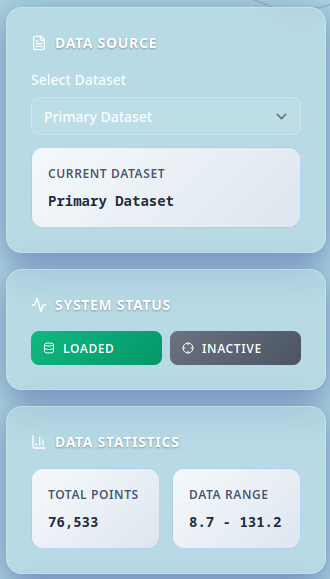
\includegraphics[width=\linewidth]{images/UI-glass-1.png}
        \caption{UI Glassmorphism 1}
        \label{fig:UI-glass-1}
    \end{subfigure}
    \qquad \qquad \qquad
    \begin{subfigure}{0.3\textwidth}
        \centering
        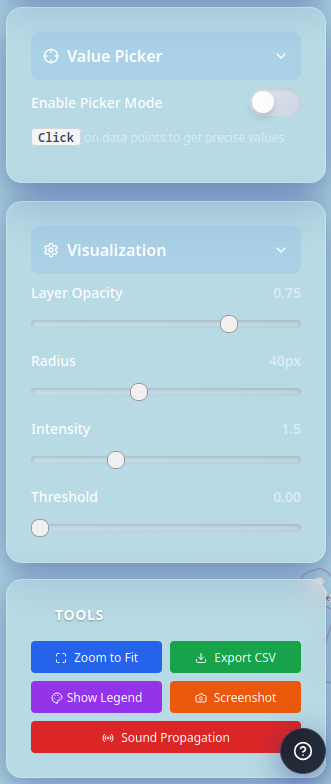
\includegraphics[width=\linewidth]{images/UI-glass-2.png}
        \caption{UI Glassmorphism 2}
        \label{fig:UI-glass-2}
    \end{subfigure}
    \caption{Esempi di Interfaccia Glassmorphism}
    \label{fig:glass-overview}
\end{figure}

\subsection{Design Responsivo}

Una delle priorità durante lo sviluppo è stata garantire la capacità del sito web di adattarsi in modo efficace al contenitore in cui viene visualizzato. La presenza congiunta di una mappa interattiva e di pannelli dotati di elementi di input eterogenei ha reso fondamentale la definizione di regole di \textit{layout} chiare e coerenti. 

Partizionare lo spazio della finestra in modo ordinato ha permesso di mantenere un'interfaccia leggibile e utilizzabile, indipendentemente dalle dimensioni dello schermo o dal livello di zoom applicato. In altre parole, l'obiettivo è stato quello di rendere l'interazione sempre fluida e accessibile, anche in condizioni di visualizzazione non ottimali.

Si è ritenuto quindi naturale l'uso di librerie in grado di portare a termine questo tipo di compito; l'intero layout è perciò basato su \textit{Tailwind CSS} ed arricchito da \textit{media queries} personalizzate, che consentono di identificare le dimensioni della finestra del browser e di conseguenza:
\begin{itemize}
  \item Ridimensionare automaticamente elementi dell'interfaccia quali griglie e container in base alla larghezza del viewport, ossia dello schermo del dispositivo utilizzato.
  \item Adattare la disposizione dei controlli per una fruizione ottimale su schermi piccoli \cite{tailwind-responsive}.
  \item Mantenere consistenza stilistica grazie alle \textit{utility class} predefinite \cite{tailwind-docs}.
\end{itemize}

Questo approccio assicura un'esperienza utente uniforme, indipendentemente dal dispositivo utilizzato.

\begin{figure}
    \centering
    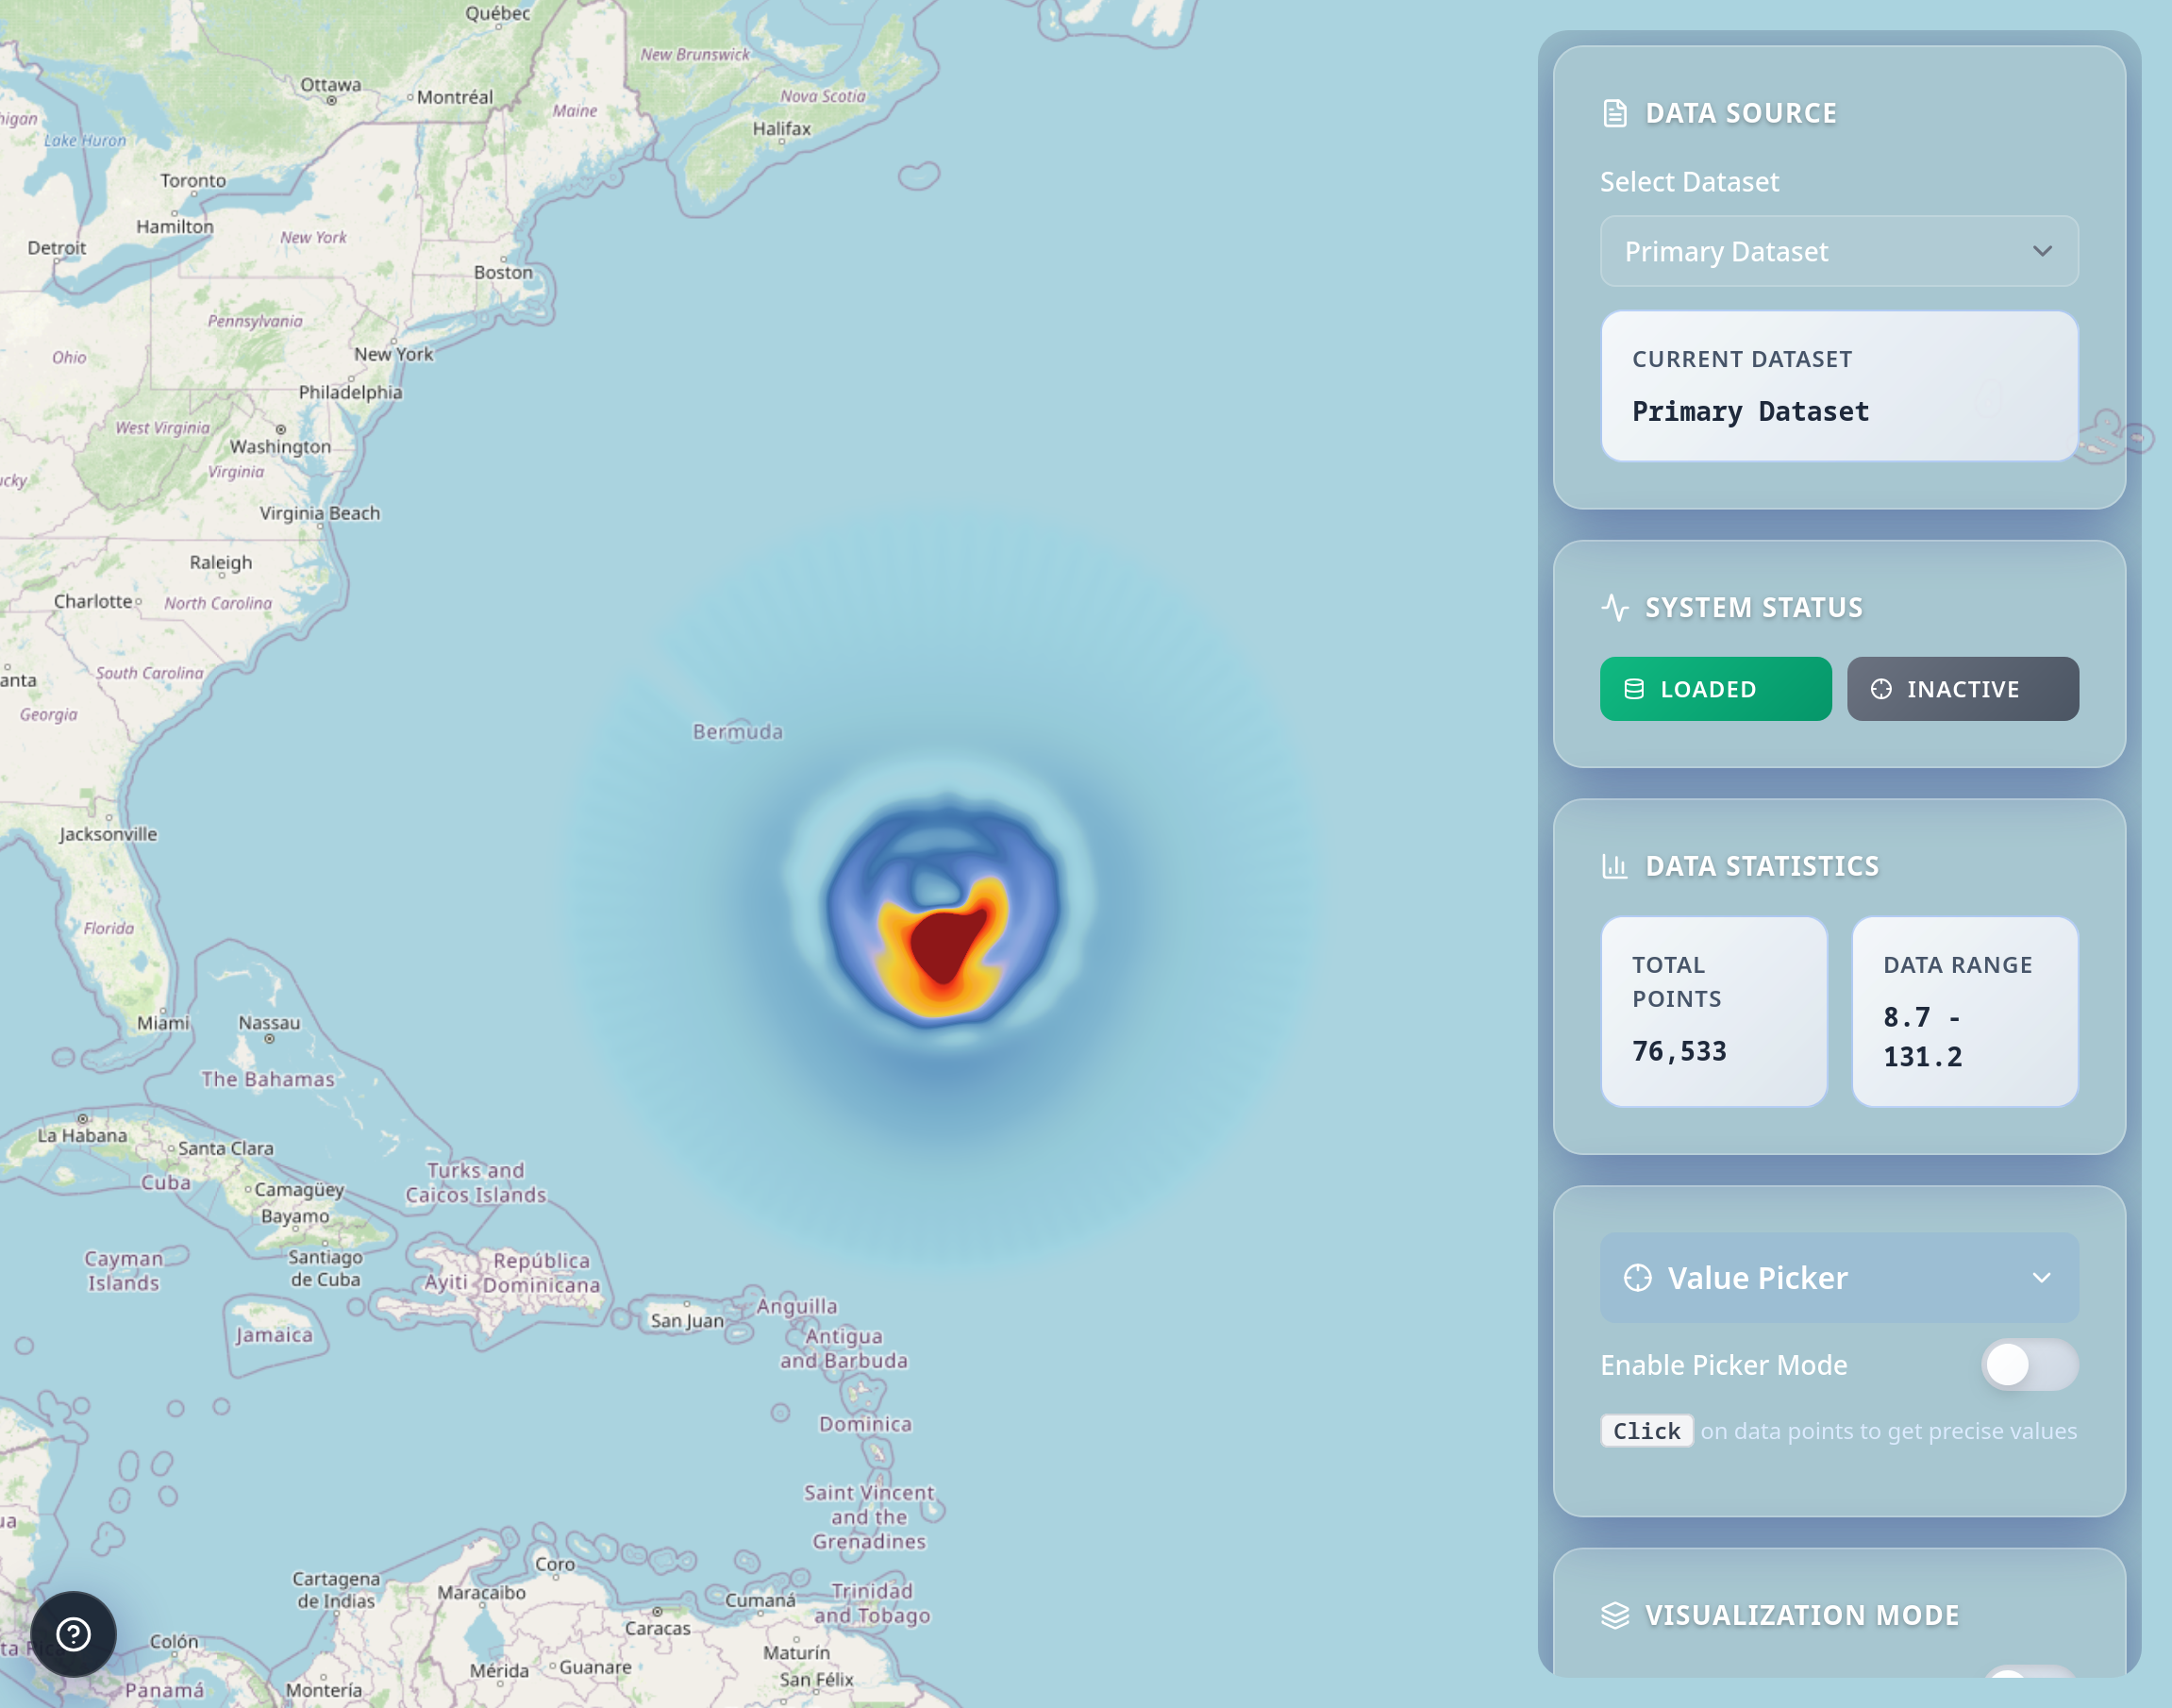
\includegraphics[width=0.86\linewidth]{images/whole-map-homepage.png}
    \caption{Interfaccia Web della Heatmap}
    \label{fig:heatmap-homepage}
\end{figure}

\subsection{Controlli Dinamici}

Per offrire un'esplorazione dei dati realmente interattiva, sono stati implementati \textit{widget} con pulsanti e slider che permettono di agire in tempo reale sulla visualizzazione (Figura \ref{fig:UI-glass-2}). Tali controlli sono in grado di variare le seguenti proprietà:

\begin{itemize}
  \item \textbf{Intensità Heatmap}: permette di regolare l'opacità della heatmap, rendendola trasparente a piacere; si utilizza per poter intravedere la mappa sottostante.
  \item \textbf{Raggio di Influenza}: Modifica la quantità di pixel su cui ogni punto influisce, variando la densità visiva delle aree.
  \item \textbf{Soglia di Visualizzazione}: Filtra i punti con valori inferiori a una soglia predefinita, eliminando il \say{rumore} dai dati.
  \item \textbf{Selezione Dataset}: Consente di passare istantaneamente tra più serie di dati, senza ricaricare l'intera pagina. (Figura \ref{fig:UI-glass-1})
\end{itemize}

Questi controlli sono collegati direttamente alle proprietà dei layer di Deck.gl, in modo da riflettere ogni modifica dell'utente senza ritardi. 
È possibile nascondere tutti i pannelli per una migliore visualizzazione della mappa sottostante tramite un apposito pulsante.

Inoltre il sistema integra un set di funzionalità progettate per ottimizzare l'interazione utente e l'analisi dei dati visualizzati. Queste caratteristiche mirano a fornire sia una visione d'insieme che un'analisi dettagliata, mantenendo al contempo un'interfaccia utente intuitiva.

\subsubsection*{Value Picker} Questa funzionalità trasforma la Heatmap in uno strumento di interrogazione precisa. Attivabile tramite un interruttore \say{Enable picker mode}, essa consente all'utente di selezionare punti specifici sulla mappa; passando con il cursore su qualsiasi punto apparirà un riquadro in cui sono indicate le coordinate geografiche (Latitudine/Longitudine) e il valore numerico esatto del punto selezionato. Tale precisione è cruciale per l'analisi puntuale dei dati. Cliccando su un punto della mappa si potranno copiare tali valori.

\subsubsection*{Statistiche Dati}
Questa sezione offre una panoramica sintetica e immediata del dataset in uso. L'elemento \say{Total Points}, che indica il numero totale di datapoint visualizzati, fornisce una stima della densità dei dati, mentre \say{Data Range} specifica l'intervallo dei valori presenti nel dataset (minimo e massimo), fornendo informazioni sulla scala dei fenomeni rappresentati.

\begin{figure}
    \centering
    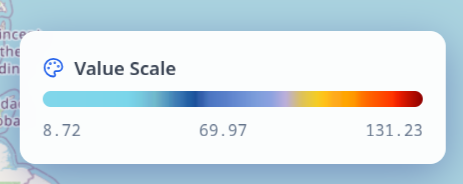
\includegraphics[width=0.5\linewidth]{images/legenda.png}
    \caption{Legenda}
    \label{fig:legenda}
\end{figure}

\subsubsection*{Legenda Colori}
Elemento interpretativo fondamentale, la Legenda Colori (in Figura \ref{fig:legenda}) facilita la comprensione del mapping tra colori e valori numerici. Caratterizzata da un \say{Gradiente dinamico}, la scala dei colori si adatta automaticamente al \say{Range valori} del dataset corrente, massimizzando la differenziazione visiva. Vi è un pulsante che permette all'utente di mostrare o nascondere la legenda per ottimizzare lo spazio o la pulizia visiva, mentre le etichette numeriche che si trovano sotto la barra colorata forniscono riferimenti chiari ai valori minimo e massimo del gradiente, essenziali per una corretta interpretazione quantitativa della Heatmap.

\subsection{Simulazione Propagazione}

Il sistema adotta un modello di propagazione acustica fondato sui principi fisici dell'acustica subacquea. La velocità di propagazione è fissata a 1481 m/s, un valore di riferimento comunemente accettato per la velocità del suono in acqua marina, corrispondente a condizioni standard di temperatura e salinità negli ambienti oceanici.

La propagazione viene modellata attraverso un'espansione concentrica, che considera sia la geometria dello spazio che le caratteristiche fisiche del mezzo. Il fronte d'onda si diffonde radialmente a partire dalla sorgente, mentre l'intensità del segnale è modulata in funzione della distanza, seguendo i principi dell'attenuazione geometrica e tenendo conto delle proprietà dissipative del mezzo, desunte dai valori di intensità contenuti nei dataset.

\begin{figure}[htbp]
    \centering
    % Primo frame
    \begin{subfigure}{0.32\textwidth}
        \centering
        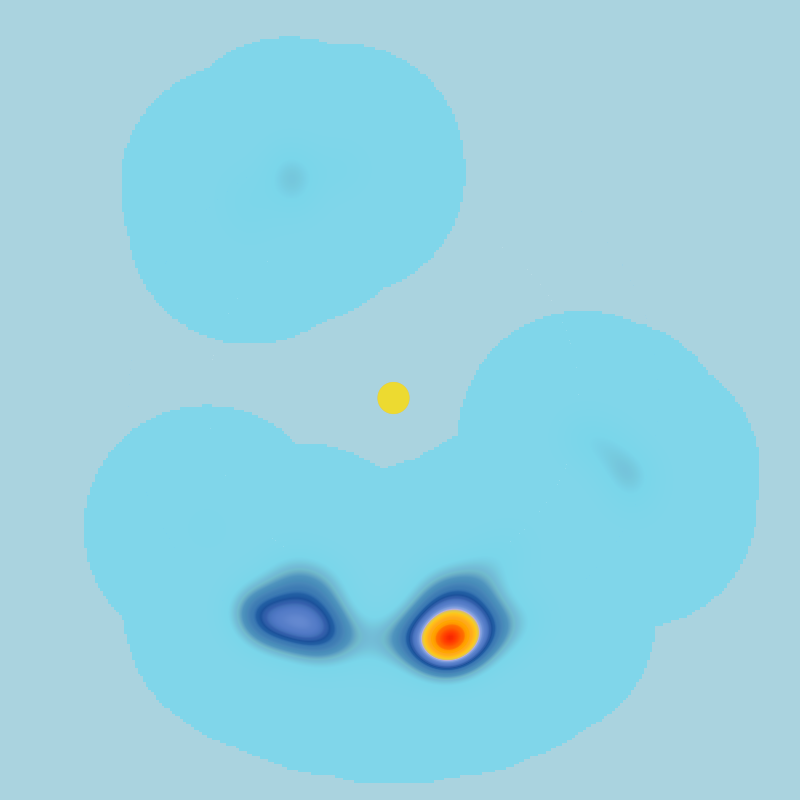
\includegraphics[width=\linewidth]{images/propagation-1.png}
        \caption{Momento iniziale} % Didascalia specifica
        \label{fig:propagation-frame-1} % Etichetta specifica
    \end{subfigure}
    \hfill % Spazio flessibile
    % Secondo frame
    \begin{subfigure}{0.32\textwidth}
        \centering
        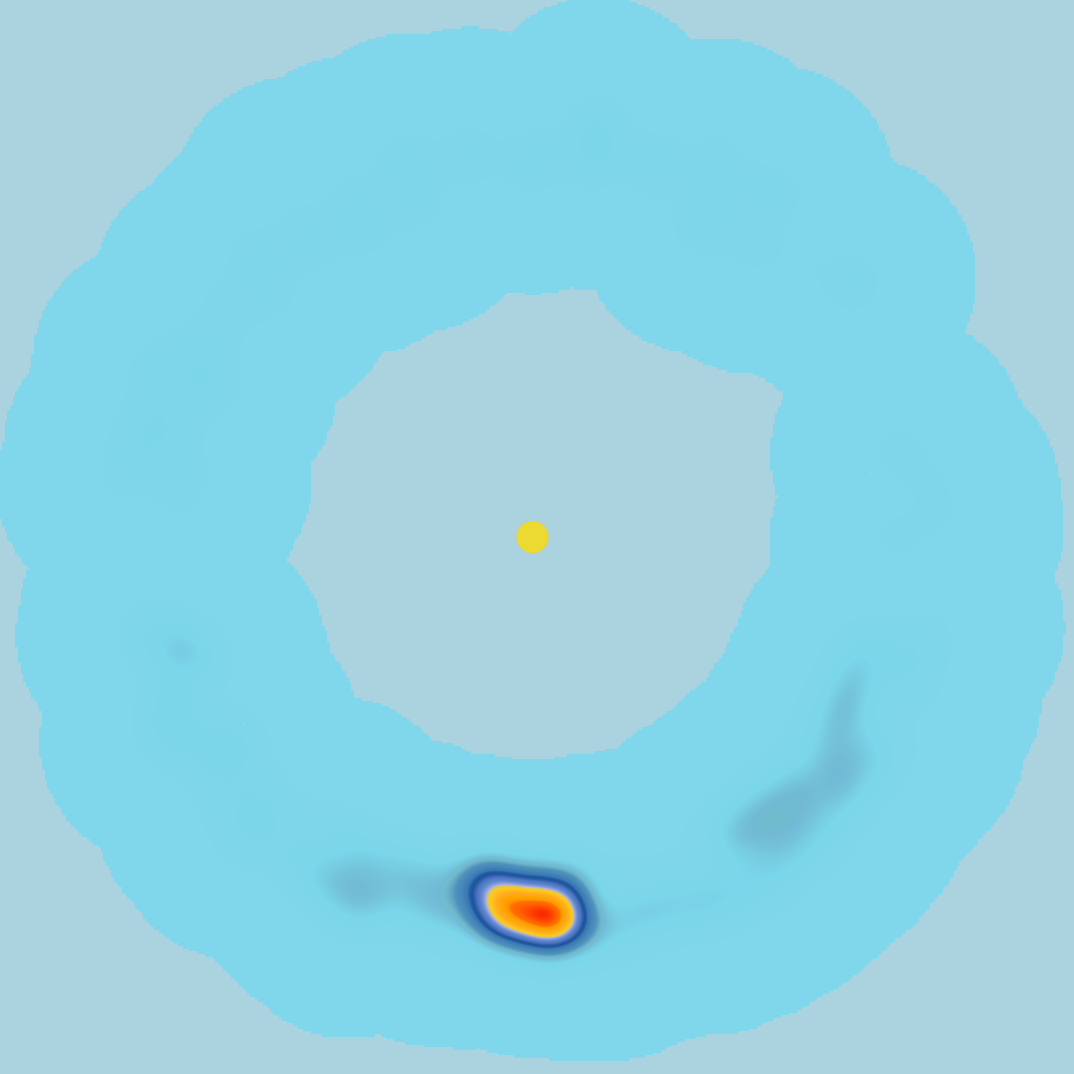
\includegraphics[width=\linewidth]{images/propagation-2.png}
        \caption{Propagazione intermedia} % Didascalia specifica
        \label{fig:propagation-frame-2} % Etichetta specifica
    \end{subfigure}
    \hfill % Spazio flessibile
    % Terzo frame
    \begin{subfigure}{0.32\textwidth}
        \centering
        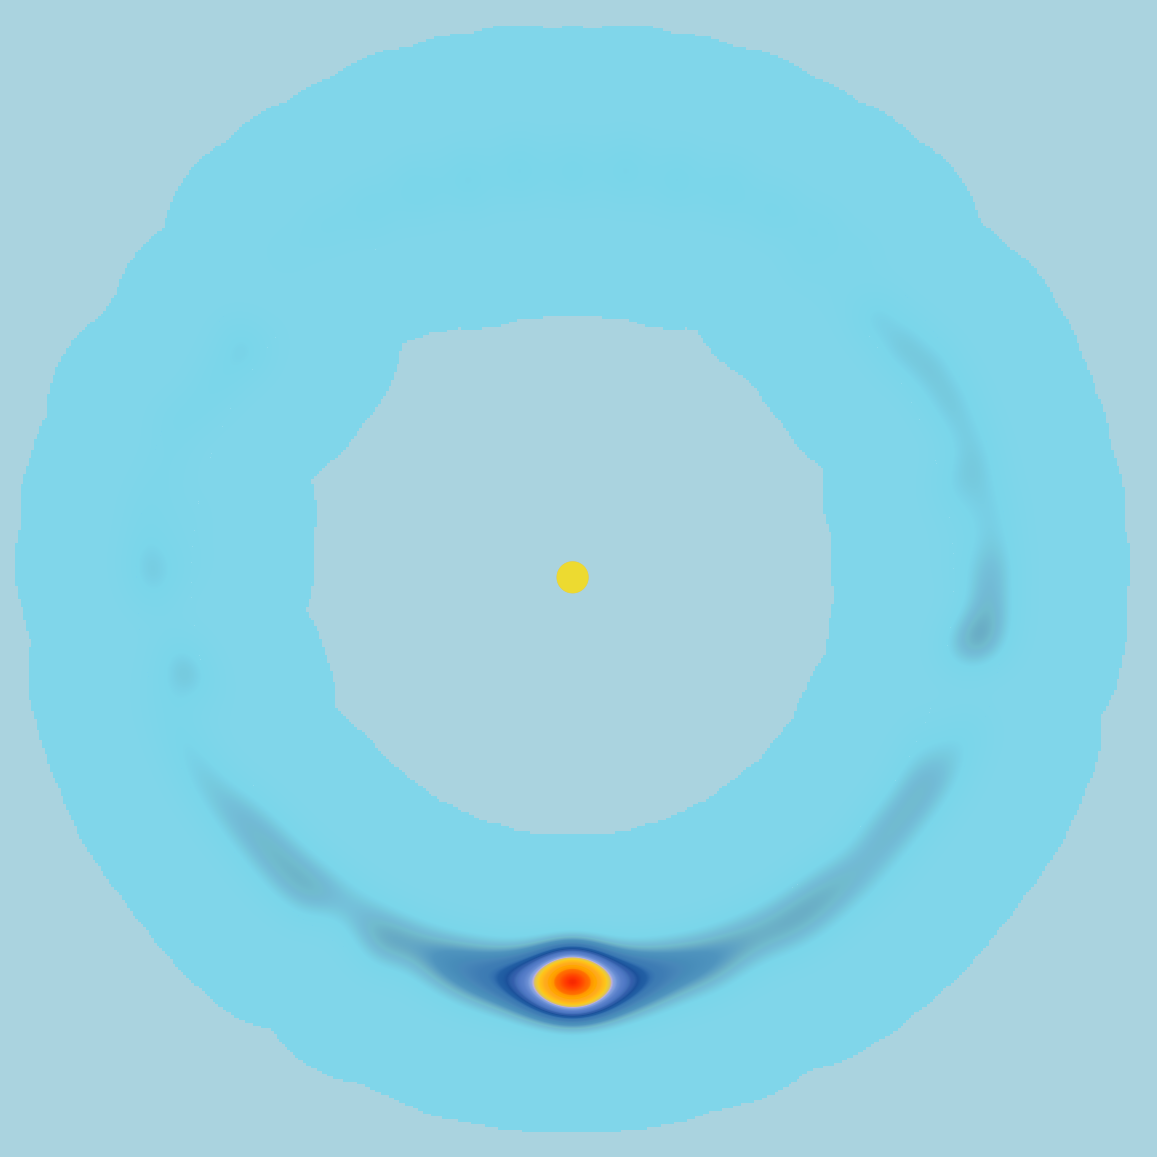
\includegraphics[width=\linewidth]{images/propagation-3.png}
        \caption{Propagazione avanzata} % Didascalia specifica
        \label{fig:propagation-frame-3} % Etichetta specifica
    \end{subfigure}
    
    \caption{Sequenza di frame illustranti l'evoluzione di un'animazione di propagazione.} % Didascalia generale
    \label{fig:propagation-animation-overview} % Etichetta generale
\end{figure}
  \chapter{Conclusioni}
\label{cha:conclusions}

\section{Sviluppi futuri}
\label{ss:sviluppi-futuri}

Il progetto costituisce un primo passo verso la creazione di un sistema integrato per la visualizzazione e l'analisi interattiva di dati geospaziali, con un focus particolare sul monitoraggio acustico marino. Dedico questa sezione all'analisi in maniera sistematica delle possibili evoluzioni del progetto, delineando sia gli sviluppi tecnici auspicabili nel breve e medio periodo, sia una roadmap di lungo termine in grado di guidare le future fasi di ricerca e sviluppo.

\subsection{Rinnovamento del Frontend}
Dal punto di vista dell'interfaccia, una migrazione a framework JavaScript moderni (come React o Vue.js) consentirebbe una maggiore modularità e manutenzione del codice. In prospettiva, il supporto a Progressive Web Apps (PWA) renderebbe l'applicazione utilizzabile anche in assenza di connessione.
L'ottimizzazione delle prestazioni grafiche passa per l'utilizzo avanzato di WebGL; in prospettiva, il supporto a WebGPU permetterebbe di sfruttare la potenza computazionale delle GPU direttamente nel browser. Aver optato per una mappa predisposta a tale tecnologia consentirà l'integrazione di WebGL senza ulteriori modifiche al codice originale.

\section{Considerazioni personali}
\label{ss:considerazioni-personali}

Lo sviluppo di questo progetto ha rappresentato per me un'occasione preziosa per approfondire tematiche legate alla visualizzazione di dati scientifici e all'ingegneria del software in ambito web. Al di là degli aspetti tecnici, ciò che ho trovato particolarmente stimolante è stato il dover progettare soluzioni non solo funzionali, ma anche usabili, robuste e sostenibili nel tempo.
\vspace{0.5em}

\noindent

Lavorare a un sistema pensato per essere importato, esteso e riutilizzato mi ha permesso di riflettere sulla necessità di scrivere codice chiaro, modulare e documentato. Ho imparato quanto sia importante definire buone astrazioni e mantenere una separazione netta tra logica di presentazione, configurazione e gestione dei dati. Inoltre, confrontarmi con strumenti avanzati di visualizzazione come \texttt{Deck.gl} mi ha aperto nuove prospettive su come i dati possano essere raccontati attraverso l'interazione visiva.

\vspace{0.5em}

\noindent

Uno degli aspetti che ho maggiormente apprezzato è stato il rapporto diretto con i dati geospaziali e ambientali. La possibilità di esplorarli in modo dinamico, adattando l'interfaccia alle esigenze di chi li consulta, mi ha fatto riflettere su come l'informatica possa facilitare la comprensione di fenomeni complessi anche al di fuori dell'ambito tecnico.

\vspace{0.5em}

\noindent
Naturalmente, non sono mancate le difficoltà: alcune scelte architetturali si sono rivelate più impegnative del previsto, e in certi casi ho dovuto modificare radicalmente l'approccio iniziale. Tuttavia, proprio in questi momenti ho avuto modo di migliorare la mia capacità di problem solving, di documentarmi in autonomia e di valutare criticamente le soluzioni disponibili.

\vspace{0.5em}

\noindent
In conclusione, considero questo lavoro non solo un'esperienza di sviluppo tecnico, ma anche un esercizio di progettazione consapevole, in cui teoria e pratica si sono intrecciate per dare vita a un sistema concreto, utile e potenzialmente riutilizzabile in altri contesti scientifici. Ne esco con una maggiore consapevolezza degli strumenti, ma anche con l'entusiasmo di continuare a imparare e contribuire a progetti complessi e multidisciplinari.

  \endgroup

  % Bibliography
  \addcontentsline{toc}{chapter}{Bibliography}
  % Alphabetical order of authors
  \bibliographystyle{plain}
  \bibliography{bibliography.bib}

  % Attachments
  % \titleformat{\chapter} {\normalfont\Huge\bfseries}{Appendix \thechapter}{1em}{}
  % \appendix
  % \chapter{GeoJSON}

\section{Introduzione}
GeoJSON è un formato aperto per lo scambio di dati geografici basato su JSON (JavaScript Object Notation) che definisce oggetti standardizzati per rappresentare entità spaziali e i loro attributi non spaziali \cite{rfc7946}. Si caratterizza per la semplicità sintattica e per l'adozione universale del sistema di riferimento WGS84, espresso in gradi decimali di longitudine e latitudine \cite{rfc7946}. La sua diffusione lo ha reso uno degli standard de facto per applicazioni web e GIS, grazie alla perfetta integrazione con librerie di mapping e piattaforme di analisi spaziale \cite{geojson-spec}.

\section{Origini e Standardizzazione}
La prima versione ufficiale di GeoJSON fu pubblicata nel 2008 sul sito geojson.org e raggiunse rapidamente una comunità di utilizzatori grazie alla sua natura testuale e leggibile \cite{geojson-first}. Successivamente, nel gennaio 2014, è stato pubblicato un Internet Draft presso l'IETF, che ha posto le basi per la standardizzazione formale \cite{geojson-first}. Infine, nell'agosto 2016, il gruppo di lavoro GeoJSON WG dell'IETF ha pubblicato la specifica definitiva come RFC 7946, sancendo la stabilità del formato e definendo regole più rigorose per le coordinate e i metadati \cite{rfc7946}.

\section{Struttura e Tipi di Geometria}
Un documento GeoJSON è un oggetto JSON che può rappresentare una singola \texttt{Feature}, una collezione di feature (\texttt{FeatureCollection}) o una \texttt{Geometry} autonoma \cite{geojson-spec}.  
I tipi di geometria supportati comprendono:
\begin{itemize}
  \item \textbf{Point}: un singolo punto con coordinate \texttt{[lon, lat]} \cite{geojson-wiki};
  \item \textbf{LineString}: una sequenza ordinata di due o più punti connessi linearmente \cite{geojson-wiki};
  \item \textbf{Polygon}: un anello chiuso di coordinate, con eventuali fori interni specificati da anelli aggiuntivi \cite{geojson-wiki};
  \item \textbf{MultiPoint}, \textbf{MultiLineString}, \textbf{MultiPolygon}: raccolte omogenee di punti, linee o poligoni \cite{geojson-wiki};
  \item \textbf{GeometryCollection}: insieme arbitrario di geometrie di vario tipo \cite{geojson-spec}.
\end{itemize}

\section{Sistema di Coordinate}
Conforme a RFC 7946, GeoJSON impiega esclusivamente il sistema di riferimento geografico WGS84 (EPSG:4326), con le coordinate espresse in gradi decimali di longitudine e latitudine \cite{rfc7946}. Non è previsto l'uso di altri sistemi di riferimento o unità di misura, per garantire interoperabilità e semplicità d'implementazione in diversi ambienti software \cite{ibm-geojson}.

\section{Feature e Proprietà}
Una \texttt{Feature} in GeoJSON associa una geometria a un insieme di proprietà non spaziali definite come coppie chiave-valore all'interno dell'oggetto \texttt{properties} \cite{geojson-spec}. Tale flessibilità consente di arricchire ogni entità geografica con informazioni descrittive, statistiche o di collegamento a risorse esterne, come URL o riferimenti a database \cite{geojson-wiki}.

\section{Applicazioni}
GeoJSON è ampiamente supportato da librerie di mapping come Leaflet e OpenLayers, che permettono di creare mappe interattive caricando direttamente file o stringhe GeoJSON \cite{leaflet-geojson,openlayers-geojson}. Il formato è altresì utilizzato da numerosi servizi di geocoding, routing e analisi spaziale, nonché da software GIS desktop quali QGIS e ArcGIS, che ne garantiscono import/export nativi \cite{arcgis-geojson}.

\section{Vantaggi e Limitazioni}
Tra i principali vantaggi di GeoJSON vi sono:
\begin{itemize}
  \item \emph{Semplicità e leggibilità}: formato testuale di rapida comprensione e modifica \cite{when-use-geojson}.
  \item \emph{Compatibilità}: supporto nativo in ogni linguaggio di programmazione che gestisca JSON \cite{geojson-spec}.
  \item \emph{Adozione diffusa}: standard de facto per il web mapping e l'interoperabilità GIS \cite{gdal-geojson}.
\end{itemize}
Le limitazioni principali interessano invece:
\begin{itemize}
  \item \emph{Scalabilità}: inefficiente per dataset di grandi dimensioni, per i quali sono preferibili formati binari come GeoPackage o TopoJSON \cite{when-use-geojson}.
  \item \emph{Ridondanza strutturale}: ripetizione di tag JSON in collezioni estese può aumentare il peso complessivo del file \cite{when-use-geojson}.
\end{itemize}

\section{Conclusioni}
GeoJSON rappresenta un equilibrio ottimale tra semplicità d'uso e potenza espressiva per la rappresentazione di dati geografici, confermandosi uno standard imprescindibile per lo sviluppo di applicazioni geospaziali sia sul web sia in ambito desktop. La sua formalizzazione in RFC 7946 ne garantisce la stabilità futura e l'interoperabilità tra piattaforme eterogenee.

\end{document}